\documentclass[12pt,a4paper]{article}

%% ---------- mathematics ----------
\usepackage{amsmath,amsthm,amssymb,mathtools}

%% ---------- graphics & diagrams ----------
\usepackage{tikz}
\usetikzlibrary{arrows.meta,positioning,shapes.geometric,calc,fit,backgrounds,matrix,decorations.pathreplacing}
\usepackage{graphicx}

%% ---------- tables ----------
\usepackage{booktabs,tabularx,multirow,longtable,array}

%% ---------- algorithms ----------
\usepackage[ruled,vlined,linesnumbered]{algorithm2e}

%% ---------- coloured boxes ----------
\usepackage[most]{tcolorbox}

%% ---------- hyperlinks & cross-refs ----------
\usepackage{hyperref}
\usepackage[capitalize,noabbrev]{cleveref}

%% ---------- page layout ----------
\usepackage[margin=1in]{geometry}
\usepackage{fancyhdr}
\usepackage{enumitem}
\usepackage{xcolor}

%% ---------- fonts & misc ----------
\usepackage{microtype}

%% ============================================================
%%  Custom tcolorbox environments
%% ============================================================
\newtcolorbox{keyinsight}[1][]{%
  colback=blue!5!white,colframe=blue!75!black,
  fonttitle=\bfseries,title=Key Insight,#1}

\newtcolorbox{example}[1][]{%
  colback=green!5!white,colframe=green!75!black,
  fonttitle=\bfseries,title=Example,#1}

\newtcolorbox{warningbox}[1][]{%
  colback=red!5!white,colframe=red!75!black,
  fonttitle=\bfseries,title=Warning,#1}

%% ============================================================
%%  amsthm environments
%% ============================================================
\newtheorem{theorem}{Theorem}[section]
\newtheorem{lemma}[theorem]{Lemma}
\newtheorem{definition}{Definition}[section]
\newtheorem{remark}{Remark}[section]
\newtheorem{proposition}[theorem]{Proposition}
\newtheorem{corollary}[theorem]{Corollary}

\pagestyle{fancy}
\fancyhf{}
\lhead{\textsc{Deep Learning} --- IIIT Dharwad}
\rhead{GRU, Sequence-to-Sequence Architecture, and Bidirectional RNN}
\rfoot{Page \thepage}
\lfoot{Prof.\ S R M Prasanna \& Dr.\ Sunil Saumya}
\renewcommand{\headrulewidth}{0.4pt}

\title{%
  {\Large\bfseries Deep Learning Course}\\[6pt]
  {\LARGE GRU, Sequence-to-Sequence Architecture, and Bidirectional RNN}\\[4pt]
  {\normalsize IIIT Dharwad --- M.Tech Programme}
}
\author{Prof.\ S R M Prasanna \& Dr.\ Sunil Saumya}
\date{Sessions 21, 22, 23}

\begin{document}

\maketitle
\tableofcontents
\clearpage

%% ============================================================
%% Session 21: Gated Recurrent Unit (GRU) and Seq2Seq Architecture
%% ============================================================
\part{Session 21: Gated Recurrent Unit (GRU) and Seq2Seq Architecture}

\begin{abstract}
These notes cover Session~21 of the deep learning course, which provides a thorough treatment of the
\textbf{Gated Recurrent Unit (GRU)}: its motivation as a simplified alternative to LSTM, the intuition
behind its two gates (reset gate $r_t$ and update gate $z_t$), its complete mathematical formulation,
a four-step numerical walkthrough, and a comparison with vanilla RNN and LSTM. The session concludes
with an introduction to the \textbf{Sequence-to-Sequence (Seq2Seq)} language model -- the foundational
architecture behind modern large language models (LLMs) -- including the encoder--decoder structure
and the role of the context vector.
\end{abstract}

\newpage

%=============================================================
\section{Introduction}
\label{sec:intro}
%=============================================================

Recurrent neural networks (RNNs) process sequential data by maintaining a hidden state that summarises
the history of the sequence seen so far.  Vanilla RNNs suffer from the \emph{vanishing/exploding
gradient} problem, which makes it difficult to capture long-range dependencies.  Long Short-Term Memory
(LSTM) networks address this limitation using a cell state $C_t$ and three learnable gates (forget,
input, output), but at the cost of a significantly higher parameter count.

The \textbf{Gated Recurrent Unit (GRU)}, proposed by Cho et al.\ (2014), offers a structurally simpler
alternative: it retains only \emph{one state line} $h_t$ (merging the separate cell state and hidden
state of LSTM) and uses \emph{two gates} instead of three.  This reduces memory and computation while
empirically matching LSTM performance on most benchmark tasks.

Session~21 also introduces the \textbf{Seq2Seq} architecture, which pairs an LSTM encoder with an LSTM
decoder connected via a fixed-size \emph{context vector}, forming the backbone of neural machine
translation and text summarisation systems.

\subsection{Learning Objectives}

After studying these notes the reader should be able to:
\begin{enumerate}[label=\arabic*.]
  \item Explain the architectural differences between RNN, LSTM, and GRU.
  \item Derive the four GRU equations from first principles.
  \item Perform a step-by-step numerical forward pass through a GRU cell.
  \item Identify how GRU gates correspond to LSTM gates.
  \item Describe the Seq2Seq encoder--decoder pipeline and its limitations.
\end{enumerate}

%=============================================================
\section{Background: From RNN to LSTM to GRU}
\label{sec:background}
%=============================================================

\subsection{Vanilla RNN Limitations}

A vanilla RNN maintains a single hidden state $h_t \in \mathbb{R}^d$ updated at each time step:
\begin{equation}
  h_t = \tanh\!\bigl(W_h\,h_{t-1} + W_x\,x_t + b\bigr).
  \label{eq:rnn}
\end{equation}
During back-propagation through time (BPTT) the gradient must pass through a chain of weight matrices.
When $\|W_h\| < 1$ the gradient vanishes; when $\|W_h\| > 1$ it explodes. In practice, dependencies
beyond 10--20 time steps are poorly captured.

\subsection{LSTM: Gating to Preserve Long-Term Context}

LSTM introduces a \emph{cell state} $C_t$ (long-term memory) alongside a hidden state $h_t$
(short-term memory) and three sigmoid gates:
\begin{align}
  f_t &= \sigma(W_f [h_{t-1}, x_t] + b_f), \label{eq:lstm_forget}\\
  i_t &= \sigma(W_i [h_{t-1}, x_t] + b_i), \label{eq:lstm_input}\\
  o_t &= \sigma(W_o [h_{t-1}, x_t] + b_o), \label{eq:lstm_output}\\
  \tilde{C}_t &= \tanh(W_C [h_{t-1}, x_t] + b_C), \label{eq:lstm_candidate}\\
  C_t &= f_t \odot C_{t-1} + i_t \odot \tilde{C}_t, \label{eq:lstm_cell}\\
  h_t &= o_t \odot \tanh(C_t). \label{eq:lstm_hidden}
\end{align}
The additive cell-state update in \cref{eq:lstm_cell} provides a gradient highway that alleviates
vanishing gradients. However, LSTM requires \emph{four} weight matrices (one per sub-network) and
\emph{two} parallel state lines, increasing both parameter count and memory footprint.

\begin{keyinsight}[title=LSTM State Summary]
LSTM uses \textbf{2 states} ($h_t$, $C_t$) and \textbf{3 gates} ($f$, $i$, $o$).
The cell state carries long-term context (LTC) and the hidden state carries short-term context (STC).
\end{keyinsight}

\subsection{Historical Note}

Interestingly, from a historical perspective the GRU was proposed \emph{before} LSTM became dominant.
As explained by Prof.\ Prasanna in Session~21:

\begin{quote}
``Initially RNN was there. When they found there is a problem in modelling the long-term context
information, they proposed GRU first, and then they segregated into LSTM. But LSTM became so prevalent
that now we study LSTM first.''
\end{quote}

%=============================================================
\section{Gated Recurrent Unit: Architecture}
\label{sec:gru_arch}
%=============================================================

\subsection{Structural Overview}

The GRU reduces LSTM complexity in two ways:
\begin{enumerate}
  \item \textbf{One state line}: $h_t$ carries both short-term context (STC) and long-term context
        (LTC) information simultaneously, with different dimensions of the vector specialised for each.
  \item \textbf{Two gates}: the reset gate $r_t$ and the update gate $z_t$ together replicate the
        combined function of LSTM's three gates.
\end{enumerate}

\cref{tab:rnn_comparison} summarises the architectural comparison.

\begin{table}[htbp]
\centering
\caption{Structural comparison of RNN, LSTM, and GRU.}
\label{tab:rnn_comparison}
\begin{tabular}{@{}lccc@{}}
\toprule
\textbf{Feature} & \textbf{RNN} & \textbf{LSTM} & \textbf{GRU} \\
\midrule
States & 1 ($h_t$) & 2 ($h_t$, $C_t$) & 1 ($h_t$) \\
Gates & 0 & 3 ($f$, $i$, $o$) & 2 ($r$, $z$) \\
Sub-networks & 1 & 4 & 3 \\
LTC / STC lines & Single (STC only) & Separate & Unified \\
Parameters & Fewest & Most & Moderate \\
Training speed & Fastest & Slowest & Intermediate \\
\bottomrule
\end{tabular}
\end{table}

\begin{keyinsight}[title=GRU Design Philosophy]
GRU merges $h_t$ and $C_t$ into a single vector. Some dimensions of $h_t$ specialise in
long-term context, while others carry short-term context. The reset and update gates
determine \emph{which dimensions are updated} at each time step.
\end{keyinsight}

\subsection{TikZ Diagram: GRU Cell}

\begin{figure}[htbp]
\centering
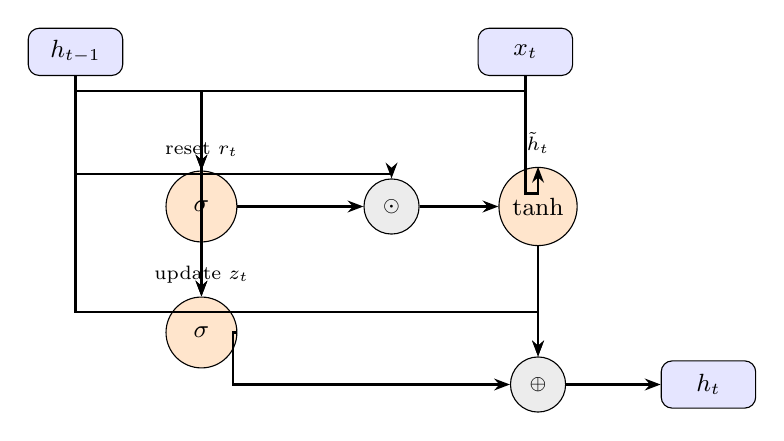
\begin{tikzpicture}[
  node distance=1.4cm and 2.0cm,
  gate/.style={draw,circle,minimum size=0.9cm,fill=orange!20,font=\small},
  op/.style={draw,circle,minimum size=0.7cm,fill=gray!15,font=\scriptsize},
  state/.style={draw,rectangle,rounded corners,minimum width=1.2cm,minimum height=0.6cm,
                fill=blue!10,font=\small},
  arr/.style={-{Stealth[length=2mm]},thick},
  every label/.style={font=\scriptsize}
]

% Inputs
\node[state] (ht1) {$h_{t-1}$};
\node[state, right=4.5cm of ht1] (xt) {$x_t$};

% Reset gate
\node[gate, below=1.2cm of ht1, xshift=1.6cm] (rgate) {$\sigma$};
\node[font=\scriptsize, above=0.05cm of rgate] {reset $r_t$};

% Update gate
\node[gate, below=2.8cm of ht1, xshift=1.6cm] (zgate) {$\sigma$};
\node[font=\scriptsize, above=0.05cm of zgate] {update $z_t$};

% Hadamard product reset * h_{t-1}
\node[op, right=1.6cm of rgate] (hadR) {$\odot$};

% Candidate tanh
\node[gate, right=1.0cm of hadR] (tanh1) {tanh};
\node[font=\scriptsize, above=0.05cm of tanh1] {$\tilde{h}_t$};

% Final blend
\node[op, below=1.4cm of tanh1] (blend) {$\oplus$};

% Output
\node[state, right=1.2cm of blend] (ht) {$h_t$};

% Arrows
\draw[arr] (ht1) -- ++(0,-0.5) -| (rgate);
\draw[arr] (xt) -- ++(0,-0.5) -| (rgate);
\draw[arr] (ht1) -- ++(0,-0.5) -| (zgate);
\draw[arr] (xt) -- ++(0,-0.5) -| (zgate);
\draw[arr] (rgate) -- (hadR);
\draw[arr] (ht1) -- ++(0,-1.55) -| (hadR);
\draw[arr] (hadR) -- (tanh1);
\draw[arr] (xt) -- ++(0,-1.8) -| (tanh1);
\draw[arr] (tanh1) -- ++(0,-0.65) -- (blend);
\draw[arr] (zgate) -- ++(0.4,0) |- (blend);
\draw[arr] (ht1) -- ++(0,-3.3) -| (blend);
\draw[arr] (blend) -- (ht);

\end{tikzpicture}
\caption{Simplified GRU cell.  The reset gate $r_t$ controls how much of the previous hidden state
feeds into the candidate; the update gate $z_t$ performs linear interpolation between the old state
and the candidate.}
\label{fig:gru_cell}
\end{figure}

%=============================================================
\section{GRU: Intuition and Notation}
\label{sec:gru_intuition}
%=============================================================

\subsection{Motivating Example: Reading a Paragraph}

\begin{example}[title=Sequential Memory in Text]
Consider the following paragraph processed token by token:
\begin{quote}
``Generative AI can generate new content. Generative AI is a type of Deep Learning.
Deep Learning is a subset of Neural Networks. Neural Networks are part of Machine Learning.''
\end{quote}
\begin{itemize}[noitemsep]
  \item When reading \emph{Generative AI} in sentence 2, the term already exists in memory -- no
        new information is needed for that token.
  \item When reading \emph{Deep Learning} for the first time, this is new information and should
        be added to memory.
  \item The word \emph{Deep Learning} reappears in sentence 3; the model may choose not to add
        it again.
  \item \emph{Neural Networks} and \emph{Machine Learning} carry new relational information.
\end{itemize}
The GRU decides at each time step: \textbf{what to remember, what to forget, and what new information
to add} -- exactly the same goal as LSTM, but with fewer parameters.
\end{example}

\subsection{Variable Notation}

\cref{tab:gru_notation} lists all variables used in the GRU formulation.

\begin{table}[htbp]
\centering
\caption{GRU variable notation at time step $t$.}
\label{tab:gru_notation}
\begin{tabular}{@{}clc@{}}
\toprule
\textbf{Symbol} & \textbf{Description} & \textbf{Range / Shape} \\
\midrule
$x_t$ & Input vector at time $t$ & $x_t \in \mathbb{R}^k$ \\
$h_{t-1}$ & Previous hidden state (memory) & $h_{t-1} \in \mathbb{R}^d$ \\
$r_t$ & Reset gate output & $r_t \in (0,1)^d$ \\
$z_t$ & Update gate output & $z_t \in (0,1)^d$ \\
$\tilde{h}_t$ & Candidate hidden state & $\tilde{h}_t \in (-1,1)^d$ \\
$h_t$ & Final hidden state & $h_t \in \mathbb{R}^d$ \\
$W_r, W_z, W$ & Learned weight matrices & $\mathbb{R}^{d \times (d+k)}$ \\
\bottomrule
\end{tabular}
\end{table}

\begin{remark}
All internal vectors $r_t$, $z_t$, $\tilde{h}_t$, and $h_t$ share the same dimension $d$,
determined by the chosen hidden size. Only $x_t$ may have a different dimension $k$.
This uniform dimensionality is required for the element-wise (Hadamard) products $\odot$.
\end{remark}

\subsection{Two-Stage Memory Update}

The GRU updates memory in exactly two stages:
\begin{equation}
  h_{t-1} \;\longrightarrow\; \tilde{h}_t \;\longrightarrow\; h_t.
  \label{eq:two_stage}
\end{equation}
Stage~1 (computing $\tilde{h}_t$) uses the \emph{reset gate} to decide how much of the old state to
``reset'' before computing a candidate. Stage~2 (computing $h_t$) uses the \emph{update gate} to
linearly interpolate between the old state and the candidate.

\begin{keyinsight}[title=Two-Stage Analogy]
Think of watching a mystery film: $h_{t-1}$ is your current belief about the plot. When a new scene
arrives ($x_t$), you first \emph{reassess} your old belief with the reset gate (perhaps forgetting
some assumptions) and form a candidate new belief $\tilde{h}_t$. Then you \emph{balance} your old
belief with the candidate via the update gate to arrive at $h_t$. You cannot rely 100\% on the
new candidate because future plot twists may reverse it.
\end{keyinsight}

%=============================================================
\section{GRU Mathematical Formulation}
\label{sec:gru_math}
%=============================================================

\subsection{The Four Core Equations}

Let $[\,h_{t-1},\,x_t\,]$ denote the concatenation of the previous hidden state and the current
input. The GRU forward pass is defined by:

\begin{align}
  z_t &= \sigma\!\bigl(W_z\cdot[h_{t-1},\,x_t]\bigr),
  \label{eq:update_gate} \\[4pt]
  r_t &= \sigma\!\bigl(W_r\cdot[h_{t-1},\,x_t]\bigr),
  \label{eq:reset_gate} \\[4pt]
  \tilde{h}_t &= \tanh\!\bigl(W\cdot[r_t \odot h_{t-1},\,x_t]\bigr),
  \label{eq:candidate} \\[4pt]
  h_t &= (1 - z_t)\odot h_{t-1} \;+\; z_t\odot\tilde{h}_t.
  \label{eq:hidden_update}
\end{align}

\cref{eq:update_gate,eq:reset_gate} each correspond to a single-layer neural network with a sigmoid
activation. They share the same input $[h_{t-1}, x_t]$ but have \emph{distinct} weight matrices
$W_z$ and $W_r$ -- this is why their outputs $z_t$ and $r_t$ differ.

\cref{eq:candidate} computes the candidate hidden state by first masking the previous hidden state
with the reset gate ($r_t \odot h_{t-1}$) before concatenating with $x_t$ and passing through
$\tanh$.

\cref{eq:hidden_update} performs a convex combination: when $z_t \approx 1$ the output is
dominated by the new candidate; when $z_t \approx 0$ the old state is preserved.

\subsection{Gate Correspondence with LSTM}

\begin{table}[htbp]
\centering
\caption{Functional mapping between GRU and LSTM gates.}
\label{tab:gate_map}
\begin{tabular}{@{}lll@{}}
\toprule
\textbf{GRU component} & \textbf{LSTM equivalent} & \textbf{Function} \\
\midrule
Reset gate $r_t$ & Forget gate $f_t$ & Selectively erase old memory \\
$(1 - z_t)$ & Input gate $i_t$ & Control new information added \\
Update gate $z_t$ & Output gate $o_t$ & Control how much to expose \\
Single state $h_t$ & Cell state $C_t$ + hidden $h_t$ & Unified LTC + STC storage \\
\bottomrule
\end{tabular}
\end{table}

\begin{warningbox}[title=Common Misconception]
The GRU does \textbf{not} simply drop one LSTM gate and keep the rest unchanged.  The update gate
$z_t$ simultaneously plays the role of the LSTM output gate, while $(1-z_t)$ acts as the input gate.
The input gate is \emph{derived} from the update gate rather than being an independent learnable
network, which is the core structural simplification.
\end{warningbox}

\subsection{Data Flow Diagram}

\begin{figure}[htbp]
\centering
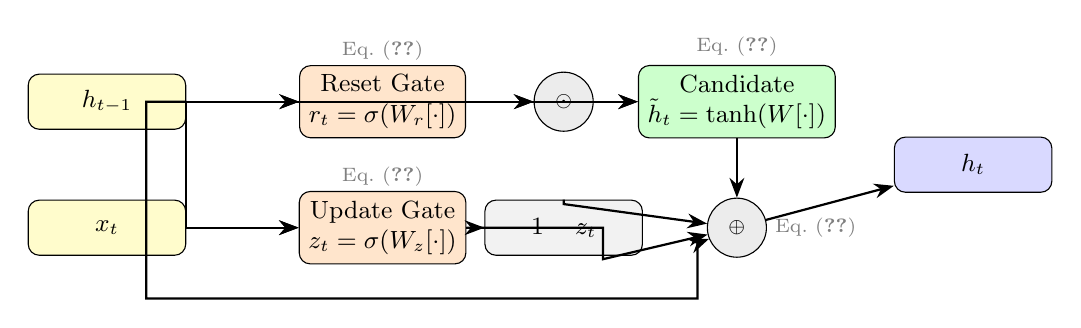
\begin{tikzpicture}[
  box/.style={draw,rounded corners,minimum width=2.0cm,minimum height=0.7cm,
              fill=yellow!20,font=\small,align=center},
  op/.style={draw,circle,minimum size=0.75cm,fill=gray!15,font=\scriptsize},
  arr/.style={-{Stealth[length=2.5mm]},thick},
  label style/.style={font=\scriptsize\itshape}
]

\node[box] (ht1)  at (0,0)   {$h_{t-1}$};
\node[box] (xt)   at (0,-1.6) {$x_t$};

% Reset gate block
\node[box,fill=orange!20] (rblock) at (3.5,0) {Reset Gate\\$r_t = \sigma(W_r[\cdot])$};
% Hadamard
\node[op] (had) at (5.8,0) {$\odot$};
% tanh
\node[box,fill=green!20] (tanhb) at (8.0,0) {Candidate\\$\tilde{h}_t = \tanh(W[\cdot])$};

% Update gate block
\node[box,fill=orange!20] (zblock) at (3.5,-1.6) {Update Gate\\$z_t = \sigma(W_z[\cdot])$};
% Blend
\node[op] (blend) at (8.0,-1.6) {$\oplus$};
% Output
\node[box,fill=blue!15] (ht) at (11.0,-0.8) {$h_t$};

% 1-z
\node[box,fill=gray!10] (onez) at (5.8,-1.6) {$1-z_t$};

% Arrows
\draw[arr] (ht1) -- (rblock);
\draw[arr] (xt) -- ++(1.0,0) |- (rblock);
\draw[arr] (rblock) -- (had);
\draw[arr] (ht1) -- ++(2.2,0) -- (had);
\draw[arr] (had) -- (tanhb);
\draw[arr] (xt) -- ++(1.0,0) |- (tanhb);
\draw[arr] (tanhb) -- ++(0,-0.5) -- (blend);

\draw[arr] (ht1) -- ++(1.0,0) |- (zblock);
\draw[arr] (xt) -- (zblock);
\draw[arr] (zblock) -- (onez);
\draw[arr] (onez) -- ++(0,0.3) -- (blend);
\draw[arr] (zblock) -- ++(2.8,0) -- ++(0,-0.4) -- (blend);
\draw[arr] (ht1) -- ++(0.5,0) -- ++(0,-2.5) -- ++(7.0,0) -- ++(0,0.7) -- (blend);
\draw[arr] (blend) -- (ht);

\node[font=\scriptsize,color=gray] at (8.0,0.7) {Eq.~(\ref*{eq:candidate})};
\node[font=\scriptsize,color=gray] at (3.5,0.65) {Eq.~(\ref*{eq:reset_gate})};
\node[font=\scriptsize,color=gray] at (3.5,-0.95) {Eq.~(\ref*{eq:update_gate})};
\node[font=\scriptsize,color=gray] at (9.0,-1.6) {Eq.~(\ref*{eq:hidden_update})};

\end{tikzpicture}
\caption{GRU data-flow diagram illustrating all four equations.  Signals from $h_{t-1}$ and $x_t$
feed both gates; the reset gate first masks $h_{t-1}$ before computing the candidate;
the update gate performs the final convex combination.}
\label{fig:gru_dataflow}
\end{figure}

\subsection{Gradient Flow Properties}

The linear interpolation in \cref{eq:hidden_update} provides an additive path for gradients:
\begin{equation}
  \frac{\partial h_t}{\partial h_{t-1}} = (1-z_t) + z_t\,\frac{\partial\tilde{h}_t}{\partial h_{t-1}}.
\end{equation}
The term $(1-z_t)$ is a direct gradient path -- analogous to the cell-state highway in LSTM --
that allows gradients to flow without being multiplied by potentially small values, thereby
mitigating vanishing gradients.

\begin{keyinsight}[title=Update Gate as Interpolation]
When $z_t = 1$, the output is entirely the new candidate $\tilde{h}_t$; when $z_t = 0$, the
output is entirely the old state $h_{t-1}$. The smooth blending prevents abrupt state overwrites
and enables stable gradient flow over long sequences.
\end{keyinsight}

%=============================================================
\section{Numerical Walkthrough}
\label{sec:numerical}
%=============================================================

This section performs a complete 4-step GRU forward pass on a concrete numerical example with
$d = 4$ (hidden dimension).

\subsection{Given Values}

\begin{align}
  h_{t-1} &= \begin{bmatrix} 0.4 \\ 0.3 \\ -0.2 \\ 0.1 \end{bmatrix},
  \quad
  x_t = \begin{bmatrix} 0.8 \\ -0.1 \\ 0.5 \\ 0.2 \end{bmatrix}.
\end{align}

\subsection{Step 1: Update Gate $z_t$}

\begin{equation}
  z_t = \sigma(W_z\cdot[h_{t-1},\,x_t])
  \;\Longrightarrow\;
  z_t = \begin{bmatrix} 0.89 \\ 0.58 \\ 0.96 \\ 0.90 \end{bmatrix}.
\end{equation}
Each element is between 0 and 1 because of the sigmoid activation.

\subsection{Step 2: Reset Gate $r_t$}

\begin{equation}
  r_t = \sigma(W_r\cdot[h_{t-1},\,x_t])
  \;\Longrightarrow\;
  r_t = \begin{bmatrix} 0.64 \\ 0.49 \\ 0.15 \\ 0.84 \end{bmatrix}.
\end{equation}
Elements close to~0 cause the corresponding dimensions of $h_{t-1}$ to be heavily suppressed,
effectively ``resetting'' those memory slots.

\subsection{Step 3: Candidate Hidden State $\tilde{h}_t$}

\begin{equation}
  \tilde{h}_t = \tanh(W\cdot[r_t\odot h_{t-1},\,x_t])
  \;\Longrightarrow\;
  \tilde{h}_t = \begin{bmatrix} 0.38 \\ 0.55 \\ -0.26 \\ 0.64 \end{bmatrix}.
\end{equation}
The $\tanh$ activation squashes values to $(-1, 1)$.

\subsection{Step 4: Final Hidden State $h_t$}

Applying \cref{eq:hidden_update}:
\begin{align}
  (1 - z_t)\odot h_{t-1}
  &= \begin{bmatrix} 0.11 \\ 0.42 \\ 0.04 \\ 0.10 \end{bmatrix},
  \qquad
  z_t \odot \tilde{h}_t
  = \begin{bmatrix} 0.34 \\ 0.32 \\ -0.25 \\ 0.58 \end{bmatrix}.
\end{align}

\begin{equation}
  \boxed{h_t = \begin{bmatrix} 0.45 \\ 0.74 \\ -0.21 \\ 0.68 \end{bmatrix}}
\end{equation}

\begin{example}[title=Interpreting the Numerical Result]
The first dimension of $h_t$ is $0.45$: this is a blend of the old value $(0.11)$ and the new
candidate $(0.34)$. The update gate value of $z_t[1] = 0.89$ means about 89\% of the new candidate
is retained, with only 11\% from the old state. For dimension 3 (index 2), $z_t[3] = 0.96$ is very
high, so the new candidate $-0.26$ dominates, giving $h_t[3] = -0.21$. This selective updating is
the core of GRU's expressiveness.
\end{example}

\subsection{Algorithm: GRU Forward Pass}

\begin{algorithm}[H]
\caption{GRU Forward Pass (single time step)}
\label{alg:gru_forward}
\DontPrintSemicolon
\KwIn{$x_t \in \mathbb{R}^k$, $h_{t-1} \in \mathbb{R}^d$,
      weight matrices $W_z, W_r, W \in \mathbb{R}^{d\times(d+k)}$}
\KwOut{$h_t \in \mathbb{R}^d$}
\BlankLine
$\text{concat} \leftarrow [h_{t-1};\, x_t]$
\tcp*{concatenate along feature axis}
\BlankLine
\tcp{Step 1: Update gate}
$z_t \leftarrow \sigma(W_z \cdot \text{concat})$\;
\BlankLine
\tcp{Step 2: Reset gate}
$r_t \leftarrow \sigma(W_r \cdot \text{concat})$\;
\BlankLine
\tcp{Step 3: Candidate hidden state}
$\text{reset\_h} \leftarrow r_t \odot h_{t-1}$\;
$\tilde{h}_t \leftarrow \tanh\!\bigl(W \cdot [\text{reset\_h};\, x_t]\bigr)$\;
\BlankLine
\tcp{Step 4: Final hidden state (convex combination)}
$h_t \leftarrow (1 - z_t)\odot h_{t-1} + z_t \odot \tilde{h}_t$\;
\BlankLine
\Return $h_t$\;
\end{algorithm}

%=============================================================
\section{GRU Across Time: Unrolled Network}
\label{sec:unrolled}
%=============================================================

Just as with vanilla RNNs and LSTMs, a GRU is applied to every element in the input sequence.
At each time step $t \in \{1, 2, \ldots, T\}$, the computation of \cref{alg:gru_forward} is
executed with the same shared weight matrices $W_z$, $W_r$, $W$.

\subsection{Parameter Count Comparison}

For hidden size $d$ and input size $k$, the number of learnable parameters is:
\begin{align}
  \text{RNN} &: \quad d(d+k) + d, \\
  \text{LSTM} &: \quad 4\bigl[d(d+k) + d\bigr], \\
  \text{GRU} &: \quad 3\bigl[d(d+k) + d\bigr].
\end{align}
GRU has 75\% of the parameters of LSTM, making it faster to train and more memory-efficient.

\begin{example}[title=Parameter Count for $d=256$, $k=512$]
\begin{align*}
  \text{LSTM parameters} &= 4 \times [256 \times (256+512) + 256]
                           = 4 \times 197\,120 = 788\,480, \\
  \text{GRU parameters}  &= 3 \times [256 \times (256+512) + 256]
                           = 3 \times 197\,120 = 591\,360.
\end{align*}
GRU saves nearly 200\,000 parameters in this configuration.
\end{example}

\subsection{When to Choose GRU vs LSTM}

There is no definitive winner between GRU and LSTM; both are used extensively in practice.
\cref{tab:gru_vs_lstm} provides practical guidance.

\begin{table}[htbp]
\centering
\caption{Practical guidance: GRU vs LSTM.}
\label{tab:gru_vs_lstm}
\begin{tabular}{@{}lcc@{}}
\toprule
\textbf{Criterion} & \textbf{LSTM} & \textbf{GRU} \\
\midrule
Very long sequences (strong LTC) & Preferred & Competitive \\
Small datasets / limited compute & Less ideal & Preferred \\
Real-time / embedded deployment & Heavier & Lighter \\
Empirical NLP benchmarks & Similar & Similar \\
Ease of implementation & More code & Simpler \\
\bottomrule
\end{tabular}
\end{table}

As noted by Prof.\ Prasanna: ``Performance-wise, there is no preference of one over the other in a
big way. The specific choice among LSTM and GRU is only in terms of complexity.''

%=============================================================
\section{Sequence-to-Sequence (Seq2Seq) Language Model}
\label{sec:seq2seq}
%=============================================================

\subsection{Motivation}

Traditional language models output a fixed-size prediction for each input token.  Many practical
tasks, however, require a \emph{variable-length output} given a \emph{variable-length input}:
\begin{itemize}[noitemsep]
  \item Neural machine translation (e.g.\ English $\to$ Hindi)
  \item Text summarisation
  \item Question answering
  \item Dialogue systems
\end{itemize}
The Seq2Seq architecture, proposed by Sutskever et al.\ (2014), addresses this by decomposing
the problem into an \textbf{encoder} and a \textbf{decoder}.

\subsection{Architecture}

\begin{definition}
A \emph{Sequence-to-Sequence model} consists of:
\begin{enumerate}[label=(\roman*)]
  \item An \textbf{encoder}: an RNN (typically LSTM or GRU) that reads the entire input sequence
        $x_1, x_2, \ldots, x_T$ and produces a fixed-size \emph{context vector} $c$.
  \item A \textbf{decoder}: an RNN conditioned on $c$ that generates the output sequence
        $y_1, y_2, \ldots, y_{T'}$ one token at a time.
\end{enumerate}
\end{definition}

\begin{figure}[htbp]
\centering
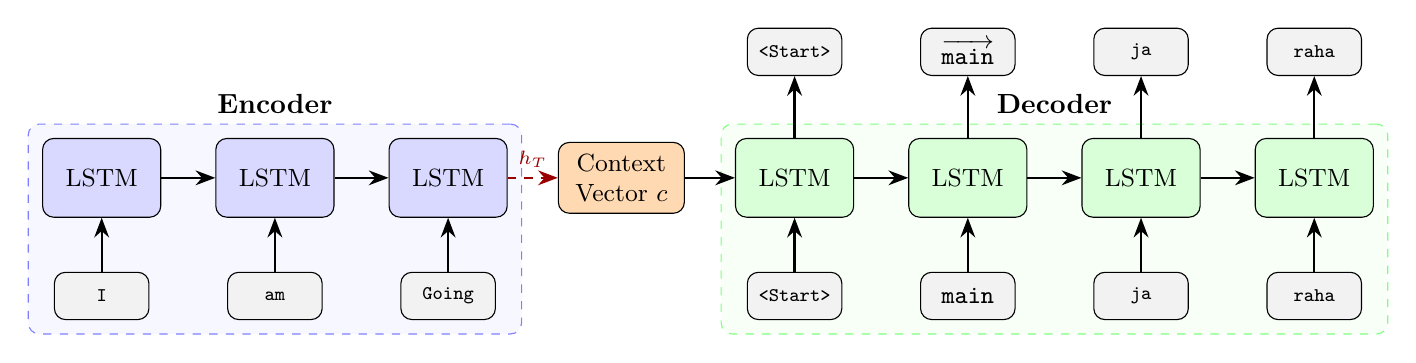
\begin{tikzpicture}[
  cell/.style={draw,rectangle,rounded corners,minimum width=1.5cm,minimum height=1.0cm,
               fill=blue!15,font=\small,align=center},
  dcell/.style={draw,rectangle,rounded corners,minimum width=1.5cm,minimum height=1.0cm,
                fill=green!15,font=\small,align=center},
  tok/.style={draw,rounded corners,minimum width=1.2cm,minimum height=0.6cm,fill=gray!10,font=\scriptsize},
  arr/.style={-{Stealth[length=2.5mm]},thick},
  darr/.style={-{Stealth[length=2.5mm]},thick,dashed,color=red!60!black}
]

% Encoder cells
\node[cell] (e1) at (0,0) {LSTM};
\node[cell] (e2) at (2.2,0) {LSTM};
\node[cell] (e3) at (4.4,0) {LSTM};

% Encoder arrows
\draw[arr] (e1) -- (e2);
\draw[arr] (e2) -- (e3);

% Encoder inputs
\node[tok] (i1) at (0,-1.5) {\texttt{I}};
\node[tok] (i2) at (2.2,-1.5) {\texttt{am}};
\node[tok] (i3) at (4.4,-1.5) {\texttt{Going}};
\draw[arr] (i1) -- (e1);
\draw[arr] (i2) -- (e2);
\draw[arr] (i3) -- (e3);

% Context vector
\node[draw,rectangle,rounded corners,minimum width=1.6cm,minimum height=0.9cm,
      fill=orange!30,font=\small,align=center] (ctx) at (6.6,0) {Context\\Vector $c$};
\draw[darr] (e3) -- (ctx) node[midway,above,font=\scriptsize]{$h_T$};

% Decoder cells
\node[dcell] (d0) at (8.8,0) {LSTM};
\node[dcell] (d1) at (11.0,0) {LSTM};
\node[dcell] (d2) at (13.2,0) {LSTM};
\node[dcell] (d3) at (15.4,0) {LSTM};

% Decoder arrows
\draw[arr] (ctx) -- (d0);
\draw[arr] (d0) -- (d1);
\draw[arr] (d1) -- (d2);
\draw[arr] (d2) -- (d3);

% Decoder outputs
\node[tok] (o0) at (8.8,1.6) {\texttt{<Start>}};
\node[tok] (o1) at (11.0,1.6) {\small\texttt{$\,\overrightarrow{\text{main}}\,$}};
\node[tok] (o2) at (13.2,1.6) {\texttt{ja}};
\node[tok] (o3) at (15.4,1.6) {\texttt{raha}};

% Decoder inputs (shifted teacher-forcing style)
\node[tok] (di1) at (8.8,-1.5) {\texttt{<Start>}};
\node[tok] (di2) at (11.0,-1.5) {\small\texttt{main}};
\node[tok] (di3) at (13.2,-1.5) {\texttt{ja}};
\node[tok] (di4) at (15.4,-1.5) {\texttt{raha}};

\draw[arr] (di1) -- (d0);
\draw[arr] (di2) -- (d1);
\draw[arr] (di3) -- (d2);
\draw[arr] (di4) -- (d3);
\draw[arr] (d0) -- (o0);
\draw[arr] (d1) -- (o1);
\draw[arr] (d2) -- (o2);
\draw[arr] (d3) -- (o3);

% Bounding boxes
\begin{scope}[on background layer]
  \node[draw=blue!50,dashed,rounded corners,fit=(e1)(e2)(e3)(i1)(i2)(i3),
        label=above:{\textbf{Encoder}},inner sep=5pt,fill=blue!3] {};
  \node[draw=green!50,dashed,rounded corners,fit=(d0)(d1)(d2)(d3)(di1)(di2)(di3)(di4),
        label=above:{\textbf{Decoder}},inner sep=5pt,fill=green!3] {};
\end{scope}

\end{tikzpicture}
\caption{Seq2Seq model for English-to-Hindi translation. The encoder (blue) processes
``I am Going'' and compresses the sequence into a context vector $c$. The decoder (green)
generates the Hindi translation token by token, conditioned on $c$.}
\label{fig:seq2seq}
\end{figure}

\subsection{Mathematical Formulation}

\textbf{Encoder:}
\begin{align}
  h_t^{\text{enc}} &= \text{LSTM}(x_t,\, h_{t-1}^{\text{enc}}), \quad t = 1,\ldots,T, \\
  c &= h_T^{\text{enc}}.
  \label{eq:context_vector}
\end{align}

\textbf{Decoder:}
\begin{align}
  s_0 &= c, \\
  s_j &= \text{LSTM}(y_{j-1},\, s_{j-1}), \quad j = 1,\ldots,T', \\
  p(y_j \mid y_{<j},\, c) &= \text{softmax}(W_s\, s_j + b_s).
\end{align}

The objective is to maximise the conditional log-likelihood:
\begin{equation}
  \mathcal{L} = \sum_{j=1}^{T'} \log p(y_j \mid y_{<j},\, c).
  \label{eq:seq2seq_loss}
\end{equation}

\subsection{Challenges}

\begin{warningbox}[title=Fixed-Size Context Vector Bottleneck]
The entire input sequence is compressed into a single fixed-size vector $c$
(see \cref{eq:context_vector}). For very long sequences this creates an
\textbf{information bottleneck}: early tokens may be poorly represented in $c$
by the time the encoder finishes. This limitation motivated the development of
\textbf{attention mechanisms} (Bahdanau et al., 2015) and eventually
\textbf{Transformers} (Vaswani et al., 2017).
\end{warningbox}

\subsection{Significance for LLMs}

As stated in the lecture: ``LLM evolution starts with the Seq2Seq model.'' The key contributions of
Seq2Seq are:
\begin{enumerate}[label=\arabic*.]
  \item Demonstrated that a single neural architecture can handle \emph{variable-length} input and
        output sequences.
  \item Introduced the \emph{encoder--decoder} paradigm that underlies T5, BART, and many
        other modern models.
  \item Motivated attention mechanisms by exposing the bottleneck of a single context vector.
\end{enumerate}

%=============================================================
\section{Comparison Summary}
\label{sec:comparison}
%=============================================================

\subsection{RNN Family Progression}

The three architectures form a progression of increasing expressiveness:
\begin{enumerate}
  \item \textbf{Vanilla RNN}: simple but suffers from vanishing gradients. No gating.
  \item \textbf{GRU}: two gates, one state; good balance of expressiveness and efficiency.
  \item \textbf{LSTM}: three gates, two states; most expressive but most costly.
\end{enumerate}

\begin{keyinsight}[title=Practical Rule of Thumb]
Start with GRU for most sequence modelling tasks. Switch to LSTM if you observe the GRU is not
capturing very long-range dependencies adequately. If computation is severely constrained, consider
GRU; if accuracy is paramount and data is abundant, LSTM is worth the extra parameters.
\end{keyinsight}

\subsection{GRU Equations at a Glance}

\begin{equation}
  \underbrace{z_t = \sigma(W_z[h_{t-1}, x_t])}_{\text{update gate}}
  \qquad
  \underbrace{r_t = \sigma(W_r[h_{t-1}, x_t])}_{\text{reset gate}}
\end{equation}
\begin{equation}
  \underbrace{\tilde{h}_t = \tanh(W[r_t\odot h_{t-1},\, x_t])}_{\text{candidate hidden state}}
\end{equation}
\begin{equation}
  \underbrace{h_t = (1-z_t)\odot h_{t-1} + z_t\odot\tilde{h}_t}_{\text{final hidden state (convex combination)}}
\end{equation}

%=============================================================
\section{Session Summary}
\label{sec:summary}
%=============================================================

Session~21 covered the following topics:

\begin{enumerate}[label=\S\arabic*.]
  \item \textbf{GRU overview}: GRU as a simplified LSTM with 1 state ($h_t$) and 2 gates
        ($r_t$, $z_t$), reducing from 4 sub-networks to 3, and from 2 state lines to 1.

  \item \textbf{Intuition}: The reset gate controls how much of the old memory is visible when
        computing the candidate; the update gate performs a smooth interpolation between old
        and new memory.

  \item \textbf{Mathematical flow}: Four equations -- update gate, reset gate, candidate hidden
        state, and final hidden state -- were derived and related to their LSTM counterparts.

  \item \textbf{Numerical walkthrough}: A 4-dimensional example was computed step by step,
        confirming the final state $h_t = [0.45, 0.74, -0.21, 0.68]^\top$ via the linear
        interpolation formula.

  \item \textbf{Gate correspondence}: GRU's reset gate $\equiv$ LSTM forget gate;
        $(1-z_t)$ $\equiv$ LSTM input gate; $z_t$ $\equiv$ LSTM output gate.

  \item \textbf{Seq2Seq introduction}: Encoder--decoder architecture using LSTM cells;
        the encoder compresses the input to a context vector $c = h_T^{\text{enc}}$, and the
        decoder generates a variable-length output sequence conditioned on $c$. Identified as
        the foundational architecture for modern LLMs.
\end{enumerate}

\subsection{Key Formulas}

\begin{align*}
  z_t &= \sigma(W_z\cdot[h_{t-1},x_t]) & \text{(update gate)}\\
  r_t &= \sigma(W_r\cdot[h_{t-1},x_t]) & \text{(reset gate)}\\
  \tilde{h}_t &= \tanh(W\cdot[r_t\odot h_{t-1},x_t]) & \text{(candidate)}\\
  h_t &= (1-z_t)\odot h_{t-1} + z_t\odot\tilde{h}_t & \text{(final state)}\\
  c &= h_T^{\text{enc}} & \text{(context vector)}
\end{align*}

\subsection{Looking Ahead}

The Seq2Seq model's fixed-size bottleneck motivates the introduction of the
\textbf{attention mechanism}: instead of using only the final encoder state $h_T$, the decoder
attends to all encoder hidden states $\{h_1, h_2, \ldots, h_T\}$ at each decoding step.
Attention is a prerequisite for understanding the Transformer architecture studied in later sessions.

\clearpage

%% ============================================================
%% Session 22: Sequence-to-Sequence Architecture and Its Limitations
%% ============================================================
\part{Session 22: Sequence-to-Sequence Architecture and Its Limitations}

% ============================================================

\begin{abstract}
This document is a comprehensive set of notes for Session~22 of the Deep Learning course at IIITDwd.
The session covers the motivation for sequence-to-sequence (Seq2Seq) models, the encoder--decoder
architecture built on LSTM units, the autoregressive inference procedure (teacher forcing vs.\ greedy
decoding), and the critical limitations that arise from compressing an entire source sequence into a
single fixed-size context vector. The final part of the session presents a hands-on PyTorch
implementation of Seq2Seq for English-to-Hindi machine translation.
These limitations directly motivate the attention mechanism introduced in Session~24.
\end{abstract}

\newpage

% ============================================================
\section{Introduction}
\label{sec:introduction}
% ============================================================

By Session~22, the course has covered three principal neural-network families:
\begin{itemize}[noitemsep]
  \item \textbf{Fully-connected (ANN)} -- suitable for tabular, fixed-length, order-independent inputs.
  \item \textbf{Convolutional (CNN)} -- designed for spatially structured data such as images; exploits
        local correlations and weight sharing.
  \item \textbf{Recurrent (RNN / LSTM / GRU)} -- tailored for sequential data where temporal ordering
        matters; maintains a hidden state that evolves over time steps.
\end{itemize}

Each family was motivated by a concrete data modality and a shortcoming of its predecessor. This
session introduces a \emph{fourth} paradigm: the \textbf{sequence-to-sequence (Seq2Seq)} model. The
central problem is that all three families above map an input of a fixed structure to an output of a
fixed structure. Real applications such as machine translation, text summarisation, and question
answering, however, require \emph{variable-length input $\to$ variable-length output} mappings -- a
regime none of the preceding architectures handles naturally.

\begin{keyinsight}
  The fundamental mismatch that Seq2Seq solves: a source sentence of length $T_x$ must be
  mapped to a target sentence of length $T_y$, where $T_x$ and $T_y$ are \emph{independent}
  and unknown at model-design time. Neither vanilla RNNs nor LSTMs provide a direct mechanism
  for this ``many-to-many with mismatched lengths'' setting.
\end{keyinsight}

The historical context is also important: the Seq2Seq architecture was proposed in 2014 in the
landmark paper ``Sequence to Sequence Learning with Neural Networks'' by Sutskever, Vinyals, and
Le~\cite{sutskever2014}. It used multi-layer LSTMs for both the encoder and decoder and achieved
state-of-the-art results on English-to-French translation at the time.

% ============================================================
\section{Background: Recap of Sequential Models}
\label{sec:background}
% ============================================================

\subsection{Vanilla RNN Limitations}

A vanilla RNN processes a sequence $\mathbf{x} = (x_1, x_2, \ldots, x_T)$ by updating a hidden
state:
\begin{equation}
  h_t = \tanh\!\left(W_{hh}\,h_{t-1} + W_{xh}\,x_t + b_h\right),
  \label{eq:rnn_hidden}
\end{equation}
where $W_{hh}$ and $W_{xh}$ are shared weight matrices. The output at each step is
$\hat{y}_t = \text{softmax}(W_{hy}\,h_t + b_y)$. Because gradients must backpropagate through
many time steps, vanilla RNNs suffer from the vanishing/exploding gradient problem and cannot
reliably capture long-range dependencies.

\subsection{LSTM: Gated Memory}

The Long Short-Term Memory (LSTM) cell addresses this by introducing explicit gating:
\begin{align}
  f_t &= \sigma\!\left(W_f [h_{t-1}, x_t] + b_f\right) & &\text{(forget gate)} \label{eq:lstm_f}\\
  i_t &= \sigma\!\left(W_i [h_{t-1}, x_t] + b_i\right) & &\text{(input gate)} \label{eq:lstm_i}\\
  \tilde{C}_t &= \tanh\!\left(W_C [h_{t-1}, x_t] + b_C\right) & &\text{(candidate cell)} \label{eq:lstm_cc}\\
  C_t &= f_t \odot C_{t-1} + i_t \odot \tilde{C}_t & &\text{(cell state update)} \label{eq:lstm_c}\\
  o_t &= \sigma\!\left(W_o [h_{t-1}, x_t] + b_o\right) & &\text{(output gate)} \label{eq:lstm_o}\\
  h_t &= o_t \odot \tanh(C_t) & &\text{(hidden state)} \label{eq:lstm_h}
\end{align}
The LSTM maintains \emph{two} memory tensors: the cell state $C_t$ (long-term memory) and the
hidden state $h_t$ (short-term / working memory). This dual-memory design allows relevant
information to persist over hundreds of time steps.

\subsection{GRU: Lighter Alternative}

The Gated Recurrent Unit (GRU) merges the two memory tensors into a single hidden state, using only
a reset gate $r_t$ and an update gate $z_t$:
\begin{align}
  r_t &= \sigma\!\left(W_r [h_{t-1}, x_t]\right), \label{eq:gru_r}\\
  z_t &= \sigma\!\left(W_z [h_{t-1}, x_t]\right), \label{eq:gru_z}\\
  \tilde{h}_t &= \tanh\!\left(W [r_t \odot h_{t-1}, x_t]\right), \label{eq:gru_htilde}\\
  h_t &= (1 - z_t) \odot h_{t-1} + z_t \odot \tilde{h}_t. \label{eq:gru_h}
\end{align}

\begin{keyinsight}
  LSTM vs.\ GRU: both architectures handle long-range dependencies comparably in practice.
  The GRU has fewer parameters (three gates vs.\ four) and typically trains faster. The choice
  between them should be made empirically: run both, compare validation accuracy, and prefer the
  lighter GRU if performance is equivalent.
\end{keyinsight}

\subsection{Comparison of Sequential Models}

\begin{table}[htbp]
  \centering
  \caption{Comparison of sequential neural-network variants.}
  \label{tab:rnn_comparison}
  \begin{tabular}{@{}lcccc@{}}
    \toprule
    \textbf{Model} & \textbf{Memory type} & \textbf{Gates} & \textbf{Params (hidden $d$)} & \textbf{Long-range capability} \\
    \midrule
    Vanilla RNN & Single $h_t$ & 0 & $\mathcal{O}(d^2)$ & Poor \\
    LSTM        & $h_t$ + $C_t$  & 4 & $\mathcal{O}(4d^2)$ & Good \\
    GRU         & Single $h_t$ & 3 & $\mathcal{O}(3d^2)$ & Good \\
    \bottomrule
  \end{tabular}
\end{table}

% ============================================================
\section{Seq2Seq Motivation}
\label{sec:motivation}
% ============================================================

\subsection{The Variable-Length Mapping Problem}

Consider English-to-Hindi translation:
\begin{center}
  \textit{``I am going''} $\;\longrightarrow\;$ \textit{``main ja raha hoon''}
\end{center}
The source has 3 tokens; the target has 4 tokens. More importantly, the correspondence is
\emph{non-monotonic}: ``going'' maps to two words (``ja raha''), and the subject ``I'' (``main'')
appears last in the Hindi sentence. A standard RNN that produces one output per input time step
cannot handle this.

\begin{example}[title={Why word-by-word translation fails}]
  Suppose we naively apply an LSTM in a one-to-one fashion, producing one Hindi token per English
  token:
  \[
    \underbrace{I}_{\text{step 1}} \to \underbrace{\text{main}}_{\hat{y}_1}, \quad
    \underbrace{\text{am}}_{\text{step 2}} \to \underbrace{?}_{\hat{y}_2}, \quad
    \underbrace{\text{going}}_{\text{step 3}} \to \underbrace{?}_{\hat{y}_3}.
  \]
  Problems: (i) ``going'' requires two Hindi words; (ii) word order differs; (iii) the model cannot
  produce the correct output for step~2 without knowing the full sentence meaning first.
  Hence word-by-word translation is fundamentally incorrect.
\end{example}

\subsection{Use Cases Requiring Seq2Seq}

\begin{table}[htbp]
  \centering
  \caption{Applications of Seq2Seq models with typical input/output length relationships.}
  \label{tab:usecases}
  \begin{tabular}{@{}llcc@{}}
    \toprule
    \textbf{Task} & \textbf{Description} & \textbf{Input length} & \textbf{Output length} \\
    \midrule
    Machine Translation & Source $\to$ target language & Variable & Different variable \\
    Text Summarisation  & Paragraph $\to$ summary      & Long ($\sim$50 words) & Short ($\sim$10 words) \\
    Question Answering  & Question + context $\to$ answer & Long & Short \\
    Speech Recognition  & Audio frames $\to$ text tokens & Very long & Short \\
    Code Generation     & Natural language $\to$ code snippet & Medium & Medium \\
    \bottomrule
  \end{tabular}
\end{table}

The key insight: the correct approach is to \emph{first encode the entire source sequence into a
compact representation}, and \emph{then decode that representation} into the target sequence one
token at a time. This encoder--decoder split is the central innovation of Seq2Seq models.

% ============================================================
\section{Encoder--Decoder Architecture}
\label{sec:architecture}
% ============================================================

\subsection{Overview}

The Seq2Seq model consists of two components:
\begin{enumerate}[noitemsep]
  \item \textbf{Encoder} -- reads the source sequence and produces a \emph{context vector}.
  \item \textbf{Decoder} -- initialised with the context vector, generates the target sequence
        token by token.
\end{enumerate}

\begin{definition}[Context Vector]
  \label{def:context_vector}
  The \emph{context vector} $\mathbf{c}$ is the final hidden state (and, for LSTM, the cell
  state) of the encoder after processing the entire source sequence:
  \[
    \mathbf{c} = \bigl(h_{T_x}^{(\text{enc})},\; C_{T_x}^{(\text{enc})}\bigr).
  \]
  It is a fixed-dimensional vector that is intended to encode the \emph{meaning} of the source
  sequence in its entirety.
\end{definition}

\subsection{TikZ Diagram: Encoder--Decoder Architecture}
\label{subsec:enc_dec_diagram}

\begin{figure}[htbp]
  \centering
  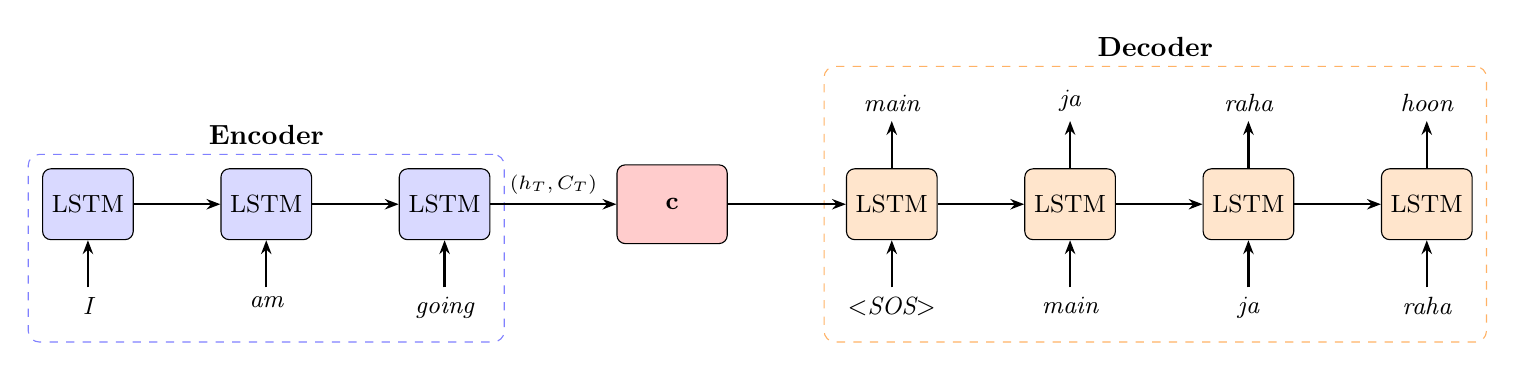
\begin{tikzpicture}[
      node distance=0.9cm and 1.1cm,
      lstm/.style={draw, rectangle, minimum width=1.1cm, minimum height=0.9cm,
                   fill=blue!15, rounded corners=3pt, font=\small},
      dlstm/.style={draw, rectangle, minimum width=1.1cm, minimum height=0.9cm,
                    fill=orange!20, rounded corners=3pt, font=\small},
      token/.style={font=\small\itshape},
      arrow/.style={-{Stealth[length=5pt]}, thick},
      cvec/.style={draw, rectangle, minimum width=1.4cm, minimum height=1.0cm,
                   fill=red!20, rounded corners=3pt, font=\small\bfseries},
    ]
    % ---- Encoder ----
    \node[lstm] (e1) {LSTM};
    \node[lstm, right=of e1] (e2) {LSTM};
    \node[lstm, right=of e2] (e3) {LSTM};

    % encoder inputs
    \node[token, below=0.6cm of e1] (w1) {I};
    \node[token, below=0.6cm of e2] (w2) {am};
    \node[token, below=0.6cm of e3] (w3) {going};

    % encoder arrows
    \draw[arrow] (w1) -- (e1);
    \draw[arrow] (w2) -- (e2);
    \draw[arrow] (w3) -- (e3);
    \draw[arrow] (e1) -- (e2);
    \draw[arrow] (e2) -- (e3);

    % context vector
    \node[cvec, right=1.6cm of e3] (cv) {$\mathbf{c}$};
    \draw[arrow] (e3) -- node[above, font=\scriptsize]{$(h_T, C_T)$} (cv);

    % ---- Decoder ----
    \node[dlstm, right=1.5cm of cv] (d1) {LSTM};
    \node[dlstm, right=of d1] (d2) {LSTM};
    \node[dlstm, right=of d2] (d3) {LSTM};
    \node[dlstm, right=of d3] (d4) {LSTM};

    % decoder inputs (bottom)
    \node[token, below=0.6cm of d1] (s0) {\textless{}SOS\textgreater};
    \node[token, below=0.6cm of d2] (t1d) {main};
    \node[token, below=0.6cm of d3] (t2d) {ja};
    \node[token, below=0.6cm of d4] (t3d) {raha};

    % decoder inputs from below
    \draw[arrow] (s0) -- (d1);
    \draw[arrow] (t1d) -- (d2);
    \draw[arrow] (t2d) -- (d3);
    \draw[arrow] (t3d) -- (d4);

    % decoder hidden connections
    \draw[arrow] (d1) -- (d2);
    \draw[arrow] (d2) -- (d3);
    \draw[arrow] (d3) -- (d4);

    % context vector to decoder init
    \draw[arrow] (cv) -- (d1);

    % decoder outputs (top)
    \node[token, above=0.6cm of d1] (o1) {main};
    \node[token, above=0.6cm of d2] (o2) {ja};
    \node[token, above=0.6cm of d3] (o3) {raha};
    \node[token, above=0.6cm of d4] (o4) {hoon};

    \draw[arrow] (d1) -- (o1);
    \draw[arrow] (d2) -- (o2);
    \draw[arrow] (d3) -- (o3);
    \draw[arrow] (d4) -- (o4);

    % bounding boxes
    \begin{scope}[on background layer]
      \node[draw=blue!50, dashed, rounded corners, fit=(e1)(e2)(e3)(w1)(w2)(w3),
            label=above:{\textbf{Encoder}}, inner sep=5pt] {};
      \node[draw=orange!60, dashed, rounded corners,
            fit=(d1)(d2)(d3)(d4)(s0)(t1d)(t2d)(t3d)(o1)(o2)(o3)(o4),
            label=above:{\textbf{Decoder}}, inner sep=5pt] {};
    \end{scope}
  \end{tikzpicture}
  \caption{Seq2Seq encoder--decoder architecture for English-to-Hindi translation.
           The encoder produces a context vector $\mathbf{c}=(h_T, C_T)$ that initialises
           the decoder. During training, teacher forcing supplies the true target tokens as
           decoder inputs; at inference, the previous prediction is fed back.}
  \label{fig:enc_dec}
\end{figure}

\subsection{Encoder Forward Pass}

Let the source sequence be $\mathbf{x} = (x_1, x_2, \ldots, x_{T_x})$. The encoder is an
$L$-layer LSTM. At each time step $t$:
\begin{align}
  \mathbf{e}_t &= E_{\text{src}}\,x_t, \label{eq:src_embed}\\
  (h_t^{(\text{enc})}, C_t^{(\text{enc})}) &= \text{LSTM}_{\text{enc}}\!\left(\mathbf{e}_t,\; h_{t-1}^{(\text{enc})},\; C_{t-1}^{(\text{enc})}\right), \label{eq:enc_step}
\end{align}
where $E_{\text{src}} \in \mathbb{R}^{d_e \times |V_{\text{src}}|}$ is the source embedding matrix.
After processing the full source, the context vector is:
\begin{equation}
  \mathbf{c} = \bigl(h_{T_x}^{(\text{enc})},\; C_{T_x}^{(\text{enc})}\bigr).
  \label{eq:context_vec}
\end{equation}

\subsection{Decoder Forward Pass}

The decoder is also an LSTM, initialised with $\mathbf{c}$. At time step $t$:
\begin{align}
  \mathbf{e}'_t &= E_{\text{tgt}}\,y_{t-1}, \label{eq:tgt_embed}\\
  (h_t^{(\text{dec})}, C_t^{(\text{dec})}) &= \text{LSTM}_{\text{dec}}\!\left(\mathbf{e}'_t,\; h_{t-1}^{(\text{dec})},\; C_{t-1}^{(\text{dec})}\right), \label{eq:dec_step}\\
  \hat{y}_t &= \text{softmax}\!\left(W_{\text{out}}\,h_t^{(\text{dec})} + b_{\text{out}}\right), \label{eq:dec_output}
\end{align}
where $y_0 = \langle\text{SOS}\rangle$ is the start-of-sequence token.

\begin{keyinsight}
  The encoder's final state $(h_{T_x}, C_{T_x})$ directly initialises the decoder's initial
  state $(h_0^{(\text{dec})}, C_0^{(\text{dec})})$. This is why the LSTM's dual-memory design
  (hidden state + cell state) is especially natural for Seq2Seq: both tensors carry complementary
  information about the encoded source.
\end{keyinsight}

% ============================================================
\section{Training: Teacher Forcing}
\label{sec:training}
% ============================================================

\subsection{Loss Function}

Training is supervised. Each example is a pair $(\mathbf{x}, \mathbf{y})$ where $\mathbf{y} =
(y_1, y_2, \ldots, y_{T_y})$ is the ground-truth target sequence. The loss is cross-entropy
summed over all decoding steps:
\begin{equation}
  \mathcal{L} = -\sum_{t=1}^{T_y} \log P\!\left(y_t \mid y_1, \ldots, y_{t-1}, \mathbf{x}\right)
              = -\sum_{t=1}^{T_y} \log \hat{y}_t[y_t],
  \label{eq:seq2seq_loss}
\end{equation}
where $\hat{y}_t[y_t]$ denotes the predicted probability of the true token $y_t$.

\subsection{Teacher Forcing}

During training, the true target token $y_{t-1}$ is fed as the decoder input at step $t$,
regardless of what the model predicted at step $t-1$. This strategy is called \textbf{teacher
forcing}:
\begin{equation}
  \text{(training)}\qquad \text{decoder input at step }t = y_{t-1}^{(\text{true})}.
  \label{eq:teacher_forcing}
\end{equation}

\begin{example}[title={Teacher Forcing for ``I am going'' $\to$ ``main ja raha hoon''}]
  Decoder steps during training:
  \begin{center}
    \begin{tabular}{@{}cccc@{}}
      \toprule
      Step $t$ & Decoder input & Predicted $\hat{y}_t$ & Ground truth $y_t$ \\
      \midrule
      1 & \textless{}SOS\textgreater & main & main \\
      2 & main (true) & ja & ja \\
      3 & ja (true) & raha & raha \\
      4 & raha (true) & hoon & hoon \\
      5 & hoon (true) & \textless{}EOS\textgreater & \textless{}EOS\textgreater \\
      \bottomrule
    \end{tabular}
  \end{center}
  At each step, the \emph{true} previous token is supplied, not the model's prediction.
  This stabilises training but creates a train--test distribution mismatch.
\end{example}

\begin{warningbox}
  \textbf{Exposure Bias:} Teacher forcing uses ground-truth tokens during training, but at
  inference the model must use its \emph{own predictions}. If the model makes an error at
  step $t$, that erroneous token is fed as input at step $t+1$, potentially compounding
  errors throughout the sequence. This train--inference gap is called \emph{exposure bias}
  and remains an active research topic (scheduled sampling, REINFORCE, etc.).
\end{warningbox}

% ============================================================
\section{Inference: Autoregressive Decoding}
\label{sec:inference}
% ============================================================

\subsection{Greedy Decoding}

At inference time, no ground-truth labels are available. The decoder operates
\emph{autoregressively}: each generated token is fed back as the input for the next step:
\begin{equation}
  y_t = \arg\max_{v \in V} P\!\left(v \mid y_1, \ldots, y_{t-1}, \mathbf{x}\right)
      = \arg\max_v \hat{y}_t[v],
  \label{eq:greedy}
\end{equation}
with $y_0 = \langle\text{SOS}\rangle$. Generation continues until the model produces
$\langle\text{EOS}\rangle$ or a maximum length is reached. Compactly:
\begin{equation}
  y_t = \text{Decoder}\!\left(y_{t-1},\; \mathbf{c}\right).
  \label{eq:autoregressive}
\end{equation}

\subsection{TikZ Diagram: Autoregressive Inference}
\label{subsec:autoregressive_diagram}

\begin{figure}[htbp]
  \centering
  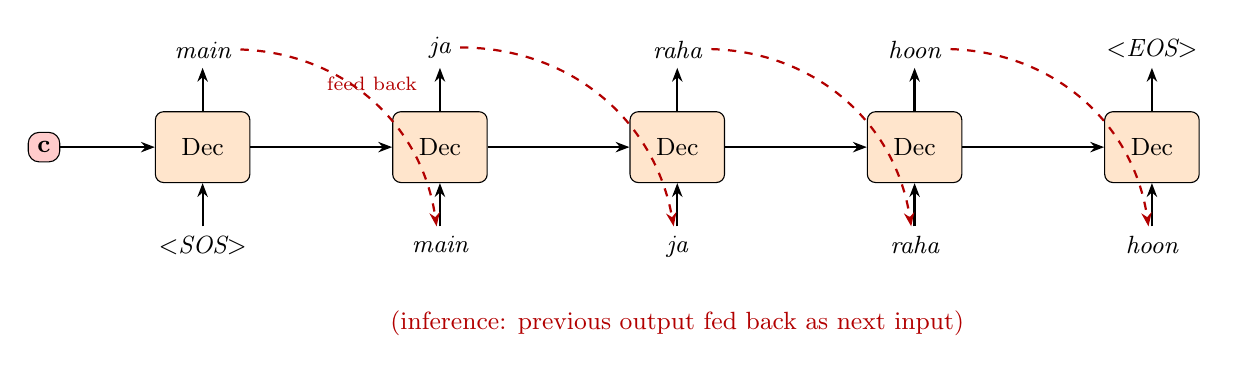
\begin{tikzpicture}[
      node distance=0.7cm and 1.2cm,
      lstm/.style={draw, rectangle, minimum width=1.2cm, minimum height=0.9cm,
                   fill=orange!20, rounded corners=3pt, font=\small},
      tok/.style={font=\small\itshape},
      arrow/.style={-{Stealth[length=5pt]}, thick},
      feedback/.style={-{Stealth[length=5pt]}, thick, dashed, bend left=40, color=red!70!black},
    ]

    \node[lstm] (d0) {Dec};
    \node[lstm, right=1.8cm of d0] (d1) {Dec};
    \node[lstm, right=1.8cm of d1] (d2) {Dec};
    \node[lstm, right=1.8cm of d2] (d3) {Dec};
    \node[lstm, right=1.8cm of d3] (d4) {Dec};

    % inputs from below
    \node[tok, below=0.55cm of d0] (i0) {\textless{}SOS\textgreater};
    \node[tok, below=0.55cm of d1] (i1) {main};
    \node[tok, below=0.55cm of d2] (i2) {ja};
    \node[tok, below=0.55cm of d3] (i3) {raha};
    \node[tok, below=0.55cm of d4] (i4) {hoon};

    % outputs above
    \node[tok, above=0.55cm of d0] (o0) {main};
    \node[tok, above=0.55cm of d1] (o1) {ja};
    \node[tok, above=0.55cm of d2] (o2) {raha};
    \node[tok, above=0.55cm of d3] (o3) {hoon};
    \node[tok, above=0.55cm of d4] (o4) {\textless{}EOS\textgreater};

    % vertical arrows
    \draw[arrow] (i0) -- (d0);
    \draw[arrow] (i1) -- (d1);
    \draw[arrow] (i2) -- (d2);
    \draw[arrow] (i3) -- (d3);
    \draw[arrow] (i4) -- (d4);

    \draw[arrow] (d0) -- (o0);
    \draw[arrow] (d1) -- (o1);
    \draw[arrow] (d2) -- (o2);
    \draw[arrow] (d3) -- (o3);
    \draw[arrow] (d4) -- (o4);

    % horizontal hidden connections
    \draw[arrow] (d0) -- (d1);
    \draw[arrow] (d1) -- (d2);
    \draw[arrow] (d2) -- (d3);
    \draw[arrow] (d3) -- (d4);

    % feedback arrows
    \draw[feedback] (o0) to node[above, font=\scriptsize\color{red!70!black}]{feed back} (i1);
    \draw[feedback] (o1) to (i2);
    \draw[feedback] (o2) to (i3);
    \draw[feedback] (o3) to (i4);

    % context vector entering d0
    \node[draw, fill=red!20, rounded corners, left=1.2cm of d0, font=\small\bfseries] (cv) {$\mathbf{c}$};
    \draw[arrow] (cv) -- (d0);

    % label
    \node[below=1.5cm of d2, font=\small\color{red!70!black}]
      {(inference: previous output fed back as next input)};
  \end{tikzpicture}
  \caption{Autoregressive decoding at inference time. The dashed red arrows show the feedback
           loop: the predicted token at step $t$ becomes the input at step $t+1$. The context
           vector $\mathbf{c}$ initialises the first decoder cell.}
  \label{fig:autoregressive}
\end{figure}

\subsection{Algorithm: Seq2Seq Inference}

\begin{algorithm}[H]
  \caption{Seq2Seq Greedy Decoding}
  \label{alg:seq2seq_inference}
  \KwIn{Source sequence $\mathbf{x} = (x_1, \ldots, x_{T_x})$; trained encoder and decoder;
        vocabulary $V$; maximum target length $T_{\max}$}
  \KwOut{Generated target sequence $\hat{\mathbf{y}}$}

  \BlankLine
  \tcp{Step 1: Encode source}
  $h_0^{(\text{enc})} \leftarrow \mathbf{0}$, $C_0^{(\text{enc})} \leftarrow \mathbf{0}$\;
  \For{$t \leftarrow 1$ \KwTo $T_x$}{
    $\mathbf{e}_t \leftarrow E_{\text{src}}\,x_t$\;
    $(h_t^{(\text{enc})}, C_t^{(\text{enc})}) \leftarrow \text{LSTM}_{\text{enc}}(\mathbf{e}_t,\, h_{t-1}^{(\text{enc})},\, C_{t-1}^{(\text{enc})})$\;
  }
  $\mathbf{c} \leftarrow (h_{T_x}^{(\text{enc})},\, C_{T_x}^{(\text{enc})})$\;

  \BlankLine
  \tcp{Step 2: Decode autoregressively}
  $h_0^{(\text{dec})} \leftarrow h_{T_x}^{(\text{enc})}$, $C_0^{(\text{dec})} \leftarrow C_{T_x}^{(\text{enc})}$\;
  $y_0 \leftarrow \langle\text{SOS}\rangle$\;
  $\hat{\mathbf{y}} \leftarrow [\;]$\;
  \For{$t \leftarrow 1$ \KwTo $T_{\max}$}{
    $\mathbf{e}'_t \leftarrow E_{\text{tgt}}\,y_{t-1}$\;
    $(h_t^{(\text{dec})}, C_t^{(\text{dec})}) \leftarrow \text{LSTM}_{\text{dec}}(\mathbf{e}'_t,\, h_{t-1}^{(\text{dec})},\, C_{t-1}^{(\text{dec})})$\;
    $\hat{y}_t \leftarrow \text{softmax}(W_{\text{out}}\,h_t^{(\text{dec})} + b_{\text{out}})$\;
    $y_t \leftarrow \arg\max_{v \in V}\;\hat{y}_t[v]$\;
    $\hat{\mathbf{y}} \leftarrow \hat{\mathbf{y}} \cup [y_t]$\;
    \If{$y_t = \langle\text{EOS}\rangle$}{\textbf{break}\;}
  }
  \Return $\hat{\mathbf{y}}$\;
\end{algorithm}

% ============================================================
\section{Limitations: The Context-Vector Bottleneck}
\label{sec:limitations}
% ============================================================

\subsection{The Bottleneck Problem}

Despite its elegance, the Seq2Seq architecture has a fundamental limitation: \textbf{all
information from the source sequence must be compressed into a single, fixed-dimensional
context vector $\mathbf{c}$}.

For short sentences this is manageable. For long sentences, the LSTM must fit an arbitrarily
long sequence of information into a vector of fixed size $d$. This creates two distinct failure
modes, one on each side of the architecture.

\begin{keyinsight}
  The context-vector bottleneck is not a failure of LSTM design but an architectural
  constraint imposed by the encoder--decoder split. No matter how large $d$ is, information
  \emph{must} be compressed. The attention mechanism, introduced in Session~24, addresses this
  by giving the decoder access to \emph{all} encoder hidden states rather than just the final
  one.
\end{keyinsight}

\subsection{Encoder-Side Problem}

When the source sentence is long, the LSTM encoder must simultaneously retain information about
early tokens and late tokens within the same fixed-size cell state $C_{T_x}$. Because gates
are applied multiplicatively:
\begin{equation}
  C_t = f_t \odot C_{t-1} + i_t \odot \tilde{C}_t,
  \label{eq:cell_overwrite}
\end{equation}
later inputs have a tendency to ``overwrite'' earlier content whenever $f_t$ is small. For a
sentence of $T_x$ tokens, the contribution of token $x_1$ to the final $C_{T_x}$ is
approximately:
\begin{equation}
  \left(\prod_{k=2}^{T_x} f_k\right) C_0 \approx 0 \quad \text{for large } T_x.
  \label{eq:forget_product}
\end{equation}
This means early words in a long source sentence tend to be forgotten by the time the encoder
finishes.

\subsection{Decoder-Side Problem}

The decoder uses \emph{the same} context vector $\mathbf{c}$ at every decoding step. There is
no mechanism for the decoder to focus on different parts of the source at different generation
steps. For example, when generating the first Hindi word the decoder ideally needs information
about the subject; when generating the verb it needs information about the verb in the source.
But $\mathbf{c}$ is static -- it cannot adapt.

\begin{remark}
  This decoder-side limitation is qualitatively different from the encoder-side one. Even if the
  encoder perfectly compressed all source information into $\mathbf{c}$, the decoder still cannot
  selectively retrieve \emph{relevant} parts of that information at each step, because
  $\mathbf{c}$ is a single undifferentiated vector.
\end{remark}

\subsection{Quantitative Summary of Limitations}

\begin{table}[htbp]
  \centering
  \caption{Summary of Seq2Seq limitations and their consequences.}
  \label{tab:limitations}
  \begin{tabular}{@{}p{3cm}p{5.5cm}p{5cm}@{}}
    \toprule
    \textbf{Location} & \textbf{Problem} & \textbf{Consequence} \\
    \midrule
    Encoder & Long sequences cannot be fully compressed into $\mathbf{c}$ & Early tokens are forgotten; quality degrades rapidly with source length \\
    \midrule
    Decoder & Same $\mathbf{c}$ used at every generation step & No dynamic focus; decoder cannot attend to relevant source tokens per step \\
    \midrule
    Both & Fixed-size bottleneck regardless of sequence complexity & Translation quality plateaus and then drops for long sentences \\
    \bottomrule
  \end{tabular}
\end{table}

\subsection{Empirical Evidence}

It was shown empirically (Cho et al., 2014~\cite{cho2014}) that BLEU scores of basic Seq2Seq
models degrade sharply once source sentences exceed roughly 20--30 words. This motivated
Bahdanau et al.\ (2015)~\cite{bahdanau2015} to introduce the attention mechanism, which
replaces the single fixed context vector with a \emph{dynamic weighted sum} over all encoder
hidden states.

% ============================================================
\section{Hands-On Implementation: PyTorch Seq2Seq}
\label{sec:implementation}
% ============================================================

\subsection{Data Preparation}

For the machine translation demo, a small English-to-Hindi corpus is used. Each example is a
pair $(\mathbf{x}_{\text{src}}, \mathbf{y}_{\text{tgt}})$ of tokenised sentences. The
vocabulary is built by iterating over all training sentences, and words are mapped to integer
indices. Special tokens are:
\begin{itemize}[noitemsep]
  \item \texttt{<PAD>} (index 0) -- padding to equalise batch lengths.
  \item \texttt{<SOS>} (index 1) -- start-of-sequence token prepended to every target.
  \item \texttt{<EOS>} (index 2) -- end-of-sequence token appended to every target.
  \item \texttt{<UNK>} (index 3) -- out-of-vocabulary words.
\end{itemize}

\subsection{Encoder Module}

The encoder wraps an \texttt{nn.Embedding} layer followed by an \texttt{nn.LSTM}:

\begin{tcolorbox}[colback=gray!5!white,colframe=gray!60!black,title=\texttt{Encoder} (PyTorch)]
\begin{verbatim}
class Encoder(nn.Module):
    def __init__(self, input_size, embedding_dim,
                 hidden_size, num_layers):
        super().__init__()
        self.embedding = nn.Embedding(input_size,
                                      embedding_dim)
        self.rnn = nn.LSTM(embedding_dim, hidden_size,
                           num_layers=num_layers,
                           batch_first=True)

    def forward(self, x):
        # x: [batch, src_len]
        embedded = self.embedding(x)
        # embedded: [batch, src_len, emb_dim]
        outputs, (hidden, cell) = self.rnn(embedded)
        # hidden: [num_layers, batch, hidden_size]
        # cell:   [num_layers, batch, hidden_size]
        return hidden, cell
\end{verbatim}
\end{tcolorbox}

Note that \texttt{outputs} (all encoder hidden states) are discarded in the basic Seq2Seq model;
only the final \texttt{(hidden, cell)} pair is used as the context vector. This is exactly
where the bottleneck arises -- all intermediate states are thrown away.

\subsection{Decoder Module}

\begin{tcolorbox}[colback=gray!5!white,colframe=gray!60!black,title=\texttt{Decoder} (PyTorch)]
\begin{verbatim}
class Decoder(nn.Module):
    def __init__(self, output_size, embedding_dim,
                 hidden_size, num_layers):
        super().__init__()
        self.embedding = nn.Embedding(output_size,
                                      embedding_dim)
        self.rnn = nn.LSTM(embedding_dim, hidden_size,
                           num_layers=num_layers,
                           batch_first=True)
        self.fc = nn.Linear(hidden_size, output_size)

    def forward(self, x, hidden, cell):
        # x: [batch] (single token per step)
        x = x.unsqueeze(1)           # [batch, 1]
        embedded = self.embedding(x) # [batch, 1, emb]
        output, (hidden, cell) = self.rnn(
            embedded, (hidden, cell))
        # output: [batch, 1, hidden_size]
        pred = self.fc(output.squeeze(1))
        # pred: [batch, output_size]
        return pred, hidden, cell
\end{verbatim}
\end{tcolorbox}

\subsection{Seq2Seq Wrapper}

\begin{tcolorbox}[colback=gray!5!white,colframe=gray!60!black,title=\texttt{Seq2Seq} (PyTorch)]
\begin{verbatim}
class Seq2Seq(nn.Module):
    def __init__(self, encoder, decoder, device):
        super().__init__()
        self.encoder = encoder
        self.decoder = decoder
        self.device  = device

    def forward(self, src, tgt,
                teacher_forcing_ratio=0.5):
        batch_size = src.shape[0]
        tgt_len    = tgt.shape[1]
        tgt_vocab  = self.decoder.fc.out_features
        outputs    = torch.zeros(batch_size,
                                 tgt_len,
                                 tgt_vocab
                                ).to(self.device)
        hidden, cell = self.encoder(src)
        x = tgt[:, 0]  # <SOS>
        for t in range(1, tgt_len):
            out, hidden, cell = \
                self.decoder(x, hidden, cell)
            outputs[:, t] = out
            teacher = random.random() < \
                          teacher_forcing_ratio
            x = tgt[:, t] if teacher \
                           else out.argmax(1)
        return outputs
\end{verbatim}
\end{tcolorbox}

\subsection{Sanity Check}

After instantiating the encoder, a quick check verifies that tensor shapes are correct:

\begin{tcolorbox}[colback=gray!5!white,colframe=gray!60!black,title=Shape Sanity Check]
\begin{verbatim}
for src_batch, tgt_batch in train_loader:
    e_h, e_c = encoder(src_batch)
    print("e_h shape:", e_h.shape)
    # Expected: [num_layers, batch_size, hidden_size]
    print("e_c shape:", e_c.shape)
    # Expected: [num_layers, batch_size, hidden_size]
    break
\end{verbatim}
\end{tcolorbox}

The shapes confirm that both the hidden state and cell state for all LSTM layers are captured in
the context vector.

\subsection{Training Loop Sketch}

Training uses cross-entropy loss ignoring padding tokens:
\begin{equation}
  \mathcal{L}_{\text{batch}} = \frac{1}{N\,T_y}
    \sum_{n=1}^{N}\sum_{t=1}^{T_y}
    \mathbf{1}[y_{n,t} \neq \text{PAD}]\cdot
    \left(-\log \hat{y}_{n,t}[y_{n,t}]\right),
  \label{eq:masked_loss}
\end{equation}
where $N$ is the batch size. The \texttt{ignore\_index} argument of
\texttt{nn.CrossEntropyLoss} handles the masking automatically.

% ============================================================
\section{Towards Attention: Motivating Session 24}
\label{sec:towards_attention}
% ============================================================

The bottleneck identified in \cref{sec:limitations} motivates a natural question: instead of
forcing the decoder to use a single static $\mathbf{c}$, why not let it access \emph{all}
encoder hidden states $(h_1^{(\text{enc})}, \ldots, h_{T_x}^{(\text{enc})})$ and compute a
\emph{dynamic, step-dependent} context?

This is precisely the attention mechanism. At each decoder step $t$, an attention score
$\alpha_{t,s}$ is computed for each encoder position $s$:
\begin{equation}
  \alpha_{t,s} = \frac{\exp(e_{t,s})}{\sum_{s'=1}^{T_x}\exp(e_{t,s'})},
  \quad e_{t,s} = \text{score}\!\left(h_t^{(\text{dec})},\, h_s^{(\text{enc})}\right),
  \label{eq:attention}
\end{equation}
and the dynamic context vector is:
\begin{equation}
  \mathbf{c}_t = \sum_{s=1}^{T_x} \alpha_{t,s}\,h_s^{(\text{enc})}.
  \label{eq:dynamic_context}
\end{equation}

\begin{example}[title={Attention in translation}]
  When decoding the Hindi verb ``ja'' from the English ``I am going'', the attention mechanism
  would ideally assign high weight to the encoder hidden state corresponding to ``going''
  ($\alpha_{t,3}$ large) and low weight to ``I'' and ``am''. This dynamic focus is impossible
  with a static context vector.
\end{example}

% ============================================================
\section{Session Summary}
\label{sec:summary}
% ============================================================

\subsection{Key Takeaways}

This session introduced the Seq2Seq encoder--decoder architecture and its LSTM-based
implementation. The main points are:

\begin{enumerate}[noitemsep]
  \item \textbf{Motivation:} Standard ANN/CNN/RNN models cannot map variable-length sequences
        to variable-length sequences. Seq2Seq addresses this with a two-phase encoder--decoder
        pipeline (proposed in 2014).

  \item \textbf{Encoder:} An LSTM reads the entire source sequence and produces a
        \emph{context vector} $(h_{T_x}, C_{T_x})$ summarising its meaning.

  \item \textbf{Decoder:} An LSTM initialised with the context vector generates the target
        sequence one token at a time via an \emph{autoregressive} process.

  \item \textbf{Training vs.\ Inference:} During training, \emph{teacher forcing} supplies
        true target tokens as decoder inputs. During inference, the model's own predictions
        are fed back, creating potential exposure bias.

  \item \textbf{Bottleneck Limitation:} Compressing an arbitrary-length source into a
        fixed-size context vector causes information loss for long sequences. The decoder
        also cannot focus on relevant source positions per step.

  \item \textbf{Motivation for Attention:} The bottleneck is resolved by providing the decoder
        with access to all encoder hidden states weighted by a learned attention distribution
        (Session~24).
\end{enumerate}

\subsection{Mathematical Notation Reference}

\begin{table}[htbp]
  \centering
  \caption{Summary of mathematical notation used in this session.}
  \label{tab:notation}
  \begin{tabular}{@{}cll@{}}
    \toprule
    \textbf{Symbol} & \textbf{Meaning} & \textbf{Dimensions} \\
    \midrule
    $h_t^{(\text{enc})}$ & Encoder hidden state at step $t$ & $\mathbb{R}^{d_h}$ \\
    $C_t^{(\text{enc})}$ & Encoder cell state at step $t$ & $\mathbb{R}^{d_h}$ \\
    $\mathbf{c}$         & Context vector (final encoder state) & $\mathbb{R}^{d_h} \times \mathbb{R}^{d_h}$ \\
    $h_t^{(\text{dec})}$ & Decoder hidden state at step $t$ & $\mathbb{R}^{d_h}$ \\
    $\hat{y}_t$          & Predicted output distribution at step $t$ & $\mathbb{R}^{|V_{\text{tgt}}|}$ \\
    $y_t$                & Predicted (or ground-truth) token at step $t$ & $\{1, \ldots, |V_{\text{tgt}}|\}$ \\
    $T_x$                & Source sequence length & -- \\
    $T_y$                & Target sequence length & -- \\
    $d_e$                & Embedding dimension & -- \\
    $d_h$                & LSTM hidden size & -- \\
    \bottomrule
  \end{tabular}
\end{table}

% ============================================================
\section{Extended Discussion: Beam Search and Evaluation}
\label{sec:beam_search}
% ============================================================

\subsection{Greedy Decoding vs.\ Beam Search}

Greedy decoding (\cref{alg:seq2seq_inference}) is fast but suboptimal: selecting the locally
best token at each step does not guarantee the globally best sequence. \textbf{Beam search}
maintains a set of $B$ candidate hypotheses (the ``beam'') and expands each by all possible
next tokens, keeping only the top-$B$ by cumulative log-probability:
\begin{equation}
  \text{score}(\mathbf{y}_{1:t}) = \sum_{k=1}^{t} \log P(y_k \mid y_1, \ldots, y_{k-1}, \mathbf{x}).
  \label{eq:beam_score}
\end{equation}
To prevent the score from favouring shorter sequences, a length penalty is often applied:
\begin{equation}
  \text{score}_{\text{norm}}(\mathbf{y}) = \frac{\text{score}(\mathbf{y})}{T_y^\alpha},
  \quad \alpha \in (0, 1].
  \label{eq:length_penalty}
\end{equation}
Typical values are $B \in \{4, 5, 10\}$ and $\alpha \approx 0.6$--$0.7$.

\subsection{BLEU Score}

The standard automatic metric for machine translation is the
\textbf{Bilingual Evaluation Understudy (BLEU)} score~\cite{papineni2002}.
BLEU measures $n$-gram precision between the hypothesis $\hat{\mathbf{y}}$ and one or more
reference translations $\mathbf{y}^{(r)}$:
\begin{equation}
  \text{BLEU} = \text{BP} \cdot \exp\!\left(\sum_{n=1}^{N} w_n \log p_n\right),
  \label{eq:bleu}
\end{equation}
where $p_n$ is the clipped $n$-gram precision, $w_n = 1/N$ (uniform weights for $N=4$), and
$\text{BP}$ is the brevity penalty:
\begin{equation}
  \text{BP} = \begin{cases} 1 & \text{if } |\hat{\mathbf{y}}| > |\mathbf{y}^{(r)}|, \\
                            e^{1 - |\mathbf{y}^{(r)}|/|\hat{\mathbf{y}}|} & \text{otherwise.}
              \end{cases}
  \label{eq:bp}
\end{equation}

\begin{warningbox}[title={BLEU Limitations}]
  BLEU is a proxy metric. It does not capture semantic adequacy, fluency beyond $n$-gram
  overlap, or handling of morphologically rich languages. Modern evaluation increasingly
  uses neural metrics such as BERTScore or ChrF, alongside human evaluation.
\end{warningbox}

% ============================================================
\section{Frequently Asked Questions from Session 22}
\label{sec:faq}
% ============================================================

The following questions arose during the live class session and are reproduced with expanded
answers.

\begin{description}[style=nextline, leftmargin=0pt]

  \item[Q: When should we use LSTM vs.\ GRU?]
    Both LSTM and GRU handle long-range dependencies comparably. The main practical difference
    is model complexity: GRU has approximately $3d^2$ parameters per layer vs.\ $4d^2$ for LSTM
    (where $d$ is the hidden size). Use GRU when training speed or model size is a constraint;
    use LSTM when you suspect the extra gating capacity may help. Always validate empirically on
    your specific task and dataset -- do not assume one is universally better.

  \item[Q: Is the context vector a single tensor or two tensors?]
    For LSTM, the context vector consists of \emph{two} tensors: the hidden state $h_{T_x}$ and
    the cell state $C_{T_x}$. Both are passed to initialise the decoder. In PyTorch, the LSTM
    returns \texttt{(hidden, cell)}, each of shape
    \texttt{[num\_layers, batch\_size, hidden\_size]}. When people informally refer to ``the
    context vector'' as a single entity, they mean this pair collectively.

  \item[Q: Why does the decoder input need a \textless{}SOS\textgreater{} token?]
    The LSTM always requires both a sequence-token input and a previous hidden state. At the
    first decoder step ($t=1$), there is no previous predicted token, so a sentinel token
    \textless{}SOS\textgreater{} is used to signal ``start decoding now.'' Its embedding is
    learnable and is effectively a ``boot'' signal for the decoder.

  \item[Q: Does the same context vector appear at every decoder step?]
    In the basic Seq2Seq model: yes. The context vector $\mathbf{c} = (h_{T_x}, C_{T_x})$ is
    used \emph{only} to initialise the decoder state at $t=0$. Thereafter, the decoder evolves
    its own hidden state. The context vector does not re-appear explicitly at steps $t > 1$.
    (Some variants concatenate $\mathbf{c}$ to every decoder input, but the original Sutskever
    et al.\ paper only uses it for initialisation.)

\end{description}

% ============================================================
% References
% ============================================================
\begin{thebibliography}{9}

\bibitem{sutskever2014}
Sutskever, I., Vinyals, O., and Le, Q.\ V. (2014).
\textit{Sequence to Sequence Learning with Neural Networks.}
Advances in Neural Information Processing Systems (NeurIPS), 27.

\bibitem{cho2014}
Cho, K., van Merri\"{e}nboer, B., Gulcehre, C., Bahdanau, D., Bougares, F.,
Schwenk, H., and Bengio, Y. (2014).
\textit{Learning Phrase Representations using RNN Encoder--Decoder for Statistical Machine Translation.}
EMNLP 2014.

\bibitem{bahdanau2015}
Bahdanau, D., Cho, K., and Bengio, Y. (2015).
\textit{Neural Machine Translation by Jointly Learning to Align and Translate.}
ICLR 2015.

\bibitem{hochreiter1997}
Hochreiter, S.\ and Schmidhuber, J. (1997).
\textit{Long Short-Term Memory.}
Neural Computation, 9(8), 1735--1780.

\bibitem{chung2014}
Chung, J., Gulcehre, C., Cho, K., and Bengio, Y. (2014).
\textit{Empirical Evaluation of Gated Recurrent Neural Networks on Sequence Modeling.}
NIPS 2014 Workshop.

\bibitem{papineni2002}
Papineni, K., Roukos, S., Ward, T., and Zhu, W.-J. (2002).
\textit{BLEU: a Method for Automatic Evaluation of Machine Translation.}
ACL 2002, pp.\ 311--318.

\bibitem{williams1989}
Williams, R.\ J.\ and Zipser, D. (1989).
\textit{A Learning Algorithm for Continually Running Fully Recurrent Neural Networks.}
Neural Computation, 1(2), 270--280.

\end{thebibliography}

\clearpage

%% ============================================================
%% Session 23: Bidirectional RNN, Stacked Seq2Seq, and Sequential Data Review
%% ============================================================
\part{Session 23: Bidirectional RNN, Stacked Seq2Seq, and Sequential Data Review}

%=============================================================

\begin{abstract}
Session 23 of the deep learning course covered three interconnected topics.
The session opened with the \emph{Bidirectional Recurrent Neural Network}
(Bi-RNN) architecture: two independent RNN (or LSTM/GRU) chains process the
input sequence in opposite directions, and each output position concatenates
the forward and backward hidden states, giving the network full past-and-future
context.  A recap of ``When Data is Sequential'' provided the RNN/LSTM/GRU
motivation within the Seq2Seq framing.  The stacked Seq2Seq architecture was
then detailed: multiple LSTM layers in both encoder and decoder increase model
capacity, with embedding layers at the input converting token IDs to dense
vectors.  The session concluded with a hands-on Google Colab walkthrough of an
English-to-Hindi machine translation pipeline --- covering tokenisation,
vocabulary construction, padding, teacher forcing, and the \texttt{Encoder}
class with a sanity check on output tensor shapes.
\end{abstract}

\newpage

\newpage

%=============================================================
\section{Introduction}
\label{sec:introduction}
%=============================================================

Recurrent Neural Networks in their simplest form process sequences strictly
from left to right.  While this \emph{unidirectional} assumption is natural for
causal prediction tasks (e.g., language modelling, real-time speech decoding),
many sequence labelling tasks benefit from knowing both the preceding and the
following context at each position.  This observation motivated the
\emph{Bidirectional RNN} (Bi-RNN)~\cite{schuster1997bidirectional}, which runs
two independent recurrent chains over the input: one in the standard
left-to-right direction, and one in the reverse right-to-left direction.

Complementing this architectural extension, \emph{Sequence-to-Sequence} (Seq2Seq)
models~\cite{sutskever2014sequence} address tasks where the output is itself a
variable-length sequence (e.g., machine translation, summarisation, question
answering).  Rather than a single recurrent network, Seq2Seq employs an
\emph{encoder} that compresses the source sequence into a fixed-size
\emph{context vector}, and a \emph{decoder} that generates the target sequence
auto-regressively from that context vector.

Session 23 unifies both threads.  After establishing the Bi-RNN formulation
(\cref{sec:birnn}), the session revisits the motivation for using recurrent
architectures with sequential data (\cref{sec:sequential}), then presents
stacked (deep) Seq2Seq models with embedding layers (\cref{sec:seq2seq}).
Finally, \cref{sec:handson} walks through the Google Colab implementation,
covering data preprocessing, tokenisation, padding, and the encoder module.

%=============================================================
\section{Background and Prerequisites}
\label{sec:background}
%=============================================================

\subsection{Vanilla Recurrent Neural Network}
\label{subsec:rnn_vanilla}

A Vanilla RNN processes a sequence $\mathbf{x} = (x_1, x_2, \ldots, x_T)$
step by step, maintaining a hidden state $h_t \in \mathbb{R}^d$ that summarises
all information seen up to time $t$:

\begin{equation}
  h_t = g\!\left(W_h\,h_{t-1} + W_x\,x_t + b\right),
  \label{eq:rnn_update}
\end{equation}

where $W_h \in \mathbb{R}^{d \times d}$, $W_x \in \mathbb{R}^{d \times n}$,
$b \in \mathbb{R}^{d}$, and $g$ is a non-linear activation (typically
$\tanh$).  The output at each time step is

\begin{equation}
  y_t = W_y\,h_t + b_y.
  \label{eq:rnn_output}
\end{equation}

\begin{remark}
  \label{rem:vanishing}
  Vanilla RNNs suffer from the \emph{vanishing gradient} problem for long
  sequences.  The gradient of the loss with respect to an early hidden state
  $h_1$ is a product of Jacobians, which tends to zero (or explodes)
  exponentially in $T$.
\end{remark}

\subsection{Long Short-Term Memory (LSTM)}
\label{subsec:lstm}

The LSTM~\cite{hochreiter1997long} mitigates the vanishing gradient by
introducing a \emph{cell state} $c_t$ and three gating mechanisms:

\begin{align}
  f_t   &= \sigma\!\left(W_f[h_{t-1}, x_t] + b_f\right),   \label{eq:lstm_f} \\
  i_t   &= \sigma\!\left(W_i[h_{t-1}, x_t] + b_i\right),   \label{eq:lstm_i} \\
  \tilde{c}_t &= \tanh\!\left(W_c[h_{t-1}, x_t] + b_c\right), \label{eq:lstm_c_tilde} \\
  c_t   &= f_t \odot c_{t-1} + i_t \odot \tilde{c}_t,       \label{eq:lstm_c} \\
  o_t   &= \sigma\!\left(W_o[h_{t-1}, x_t] + b_o\right),   \label{eq:lstm_o} \\
  h_t   &= o_t \odot \tanh(c_t).                            \label{eq:lstm_h}
\end{align}

\begin{keyinsight}
  The LSTM cell state $c_t$ flows through the network with only additive
  interactions, enabling gradients to propagate across many time steps without
  vanishing.  This property is crucial for long-sequence tasks such as machine
  translation.
\end{keyinsight}

\subsection{Gated Recurrent Unit (GRU)}
\label{subsec:gru}

The GRU~\cite{cho2014learning} simplifies LSTM by merging the forget and input
gates into a single \emph{update gate} $z_t$:

\begin{align}
  z_t &= \sigma\!\left(W_z[h_{t-1}, x_t]\right), \label{eq:gru_z} \\
  r_t &= \sigma\!\left(W_r[h_{t-1}, x_t]\right), \label{eq:gru_r} \\
  \tilde{h}_t &= \tanh\!\left(W[r_t \odot h_{t-1}, x_t]\right), \label{eq:gru_h_tilde} \\
  h_t &= (1 - z_t) \odot h_{t-1} + z_t \odot \tilde{h}_t. \label{eq:gru_h}
\end{align}

%=============================================================
\section{When Data is Sequential}
\label{sec:sequential}
%=============================================================

The slide ``When Data is Sequential: RNN / LSTM / GRU'' (Deck \texttt{10-Seq2Seq},
slide 6/25) distils the motivation for recurrent architectures into three
properties:

\begin{enumerate}[label=\textbf{P\arabic*.}]
  \item \textbf{Order matters.}  Changing the order of tokens in a sentence
        changes its meaning entirely.  A standard feed-forward network treats
        inputs as an unordered set.
  \item \textbf{Variable-length input.}  Natural language sentences, speech
        frames, and time-series windows differ in length.  RNNs handle arbitrary
        lengths naturally through weight sharing across time steps.
  \item \textbf{Context depends on previous elements.}  The hidden state
        $h_t$ in \cref{eq:rnn_update} acts as a running summary of all tokens
        seen so far, enabling the model to exploit long-range dependencies.
\end{enumerate}

\begin{figure}[h]
\centering
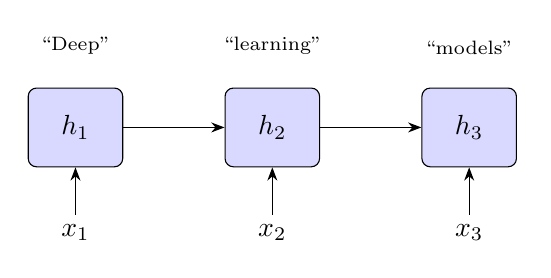
\begin{tikzpicture}[
  cell/.style={rectangle, draw, fill=blue!15, minimum width=1.2cm,
               minimum height=1.0cm, rounded corners=3pt},
  >=Stealth
]
  % Input tokens
  \node[cell] (h1) at (0,0)   {$h_1$};
  \node[cell] (h2) at (2.5,0) {$h_2$};
  \node[cell] (h3) at (5.0,0) {$h_3$};

  % Input arrows
  \node[below=0.6cm of h1] (x1) {$x_1$};
  \node[below=0.6cm of h2] (x2) {$x_2$};
  \node[below=0.6cm of h3] (x3) {$x_3$};
  \draw[->] (x1) -- (h1);
  \draw[->] (x2) -- (h2);
  \draw[->] (x3) -- (h3);

  % Recurrent arrows
  \draw[->] (h1) -- (h2);
  \draw[->] (h2) -- (h3);

  % Labels
  \node[above=0.3cm of h1, font=\scriptsize] {``Deep''};
  \node[above=0.3cm of h2, font=\scriptsize] {``learning''};
  \node[above=0.3cm of h3, font=\scriptsize] {``models''};
\end{tikzpicture}
\caption{Unidirectional RNN processing the sentence
         ``Deep learning models process sequences''.  The hidden state at each
         step summarises all preceding tokens.}
\label{fig:unidirectional_rnn}
\end{figure}

\begin{example}[title=Ambiguity Resolution with Context]
  Consider the sentence \emph{``I went to the bank to deposit money.''}
  At the moment of processing the word \emph{bank}, a left-to-right RNN
  has not yet seen \emph{``deposit money''}.  The word is ambiguous between
  a financial institution and a river bank.  If a right-to-left context is
  also available (carrying the information \emph{``deposit money''}), the
  ambiguity is resolved immediately.  This is precisely the motivation for
  Bidirectional RNNs.
\end{example}

\subsection{When Bidirectionality is Unsuitable}
\label{subsec:unsuitable}

Bidirectionality requires the \emph{complete} sequence to be available before
processing.  The following tasks are therefore unsuitable for Bi-RNNs:

\begin{itemize}
  \item \textbf{Next-word (language) modelling.}  At test time, the future
        tokens are not available; a backward pass cannot be computed.
        BERT (Bidirectional Encoder Representations from Transformers) addresses
        this by using a \emph{masked language modelling} objective instead of
        straightforward next-token prediction.
  \item \textbf{Online / streaming speech decoding.}  Speech signals evolve
        causally.  A backward pass would require buffering the entire utterance,
        introducing unacceptable latency.
\end{itemize}

\begin{keyinsight}
  The distinction between \emph{encoder}-type models (which can be
  bidirectional) and \emph{decoder}-type models (which must be causal) is
  central to the transformer literature.  BERT is a bidirectional encoder;
  GPT-style models are unidirectional decoders.
\end{keyinsight}

%=============================================================
\section{Bidirectional Recurrent Neural Networks}
\label{sec:birnn}
%=============================================================

\subsection{Architecture}
\label{subsec:birnn_arch}

A Bidirectional RNN runs two separate recurrent chains over the same input
sequence simultaneously:

\begin{enumerate}
  \item A \textbf{forward chain} processes tokens from $t=1$ to $t=T$,
        producing forward hidden states $\overrightarrow{h}_t$.
  \item A \textbf{backward chain} processes tokens from $t=T$ to $t=1$,
        producing backward hidden states $\overleftarrow{h}_t$.
\end{enumerate}

The output at position $t$ is the \emph{concatenation} of both states:

\begin{equation}
  y_t = \left[\overrightarrow{h}_t;\;\overleftarrow{h}_t\right]
        \in \mathbb{R}^{2d}.
  \label{eq:birnn_output}
\end{equation}

\cref{fig:birnn} illustrates the full architecture as shown in the lecture
slides (Deck \texttt{05-DL-RNN}, slide 74/109).

\begin{figure}[ht]
\centering
\begin{tikzpicture}[
  fwd/.style={rectangle, draw, fill=green!25, minimum width=1.1cm,
              minimum height=0.9cm, rounded corners=3pt, font=\small},
  bwd/.style={rectangle, draw, fill=orange!25, minimum width=1.1cm,
              minimum height=0.9cm, rounded corners=3pt, font=\small},
  out/.style={rectangle, draw, fill=gray!15, minimum width=1.1cm,
              minimum height=0.7cm, font=\scriptsize},
  >=Stealth, node distance=2.2cm
]
  % ---- Forward cells (bottom row) ----
  \node[fwd] (A0)  at (0,0)    {$A$};
  \node[fwd] (A1)  at (2.4,0)  {$A$};
  \node[fwd] (A2)  at (4.8,0)  {$A$};
  \node[fwd] (AT)  at (7.8,0)  {$A$};

  % ---- Backward cells (top row) ----
  \node[bwd] (B0)  at (0,2.2)   {$A'$};
  \node[bwd] (B1)  at (2.4,2.2) {$A'$};
  \node[bwd] (B2)  at (4.8,2.2) {$A'$};
  \node[bwd] (BT)  at (7.8,2.2) {$A'$};

  % ---- Inputs (below forward row) ----
  \foreach \i/\lbl in {0/$x_0$, 1/$x_1$, 2/$x_2$}{
    \pgfmathtruncatemacro{\xpos}{\i}
    \node[below=0.65cm of A\xpos] (x\i) {\lbl};
    \draw[->] (x\i) -- (A\xpos);
    \draw[->] (x\i) -- (B\xpos);
  }
  \node[below=0.65cm of AT] (xT) {$x_T$};
  \draw[->] (xT) -- (AT);
  \draw[->] (xT) -- (BT);

  % ---- Outputs (above backward row) ----
  \foreach \i in {0,1,2}{
    \node[out, above=0.65cm of B\i] (y\i) {$y_\i$};
    \draw[->] (B\i) -- (y\i);
    \draw[->] (A\i) -- (y\i);
  }
  \node[out, above=0.65cm of BT] (yT) {$y_T$};
  \draw[->] (BT) -- (yT);
  \draw[->] (AT) -- (yT);

  % ---- Forward recurrent arrows ----
  \draw[->] (A0) -- node[below,font=\scriptsize]{$s_0$} (A1);
  \draw[->] (A1) -- (A2);
  \draw[dashed,->] (A2) -- (AT);
  \node[left=0.5cm of A0, font=\scriptsize] {$s_0$};
  \node[right=0.4cm of AT, font=\scriptsize] {$s_T$};

  % ---- Backward recurrent arrows ----
  \draw[<-] (B0) -- node[above,font=\scriptsize]{} (B1);
  \draw[<-] (B1) -- (B2);
  \draw[dashed,<-] (B2) -- (BT);
  \node[left=0.5cm of B0, font=\scriptsize] {$s'_1$};
  \node[right=0.4cm of BT, font=\scriptsize] {$s'_0$};

  % ---- Ellipsis between A2/B2 and AT/BT ----
  \node at (6.3,0)   {\ldots};
  \node at (6.3,2.2) {\ldots};

  % ---- Legend ----
  \begin{scope}[shift={(0,-2.2)}]
    \node[fwd, minimum width=0.7cm] (lf) at (1,0) {$A$};
    \node[right=0.1cm of lf, font=\small] {Forward (left $\to$ right)};
    \node[bwd, minimum width=0.7cm] (lb) at (5,0) {$A'$};
    \node[right=0.1cm of lb, font=\small] {Backward (right $\to$ left)};
  \end{scope}
\end{tikzpicture}
\caption{Bidirectional RNN architecture (Deck \texttt{05-DL-RNN}, slide 74/109).
         Each output $y_t$ combines both forward and backward hidden states via
         concatenation.  Green cells ($A$) carry state left-to-right;
         orange cells ($A'$) carry state right-to-left.}
\label{fig:birnn}
\end{figure}

\subsection{Forward and Backward Equations}
\label{subsec:birnn_equations}

The forward and backward passes are independent recurrences sharing only the
input $x_t$:

\begin{align}
  \overrightarrow{h}_t &= g\!\left(
      W_{\overrightarrow{h}}\,\overrightarrow{h}_{t-1}
      + W_{\overrightarrow{x}}\,x_t + b_{\overrightarrow{h}}\right),
      \label{eq:birnn_fwd} \\[4pt]
  \overleftarrow{h}_t &= g\!\left(
      W_{\overleftarrow{h}}\,\overleftarrow{h}_{t+1}
      + W_{\overleftarrow{x}}\,x_t + b_{\overleftarrow{h}}\right).
      \label{eq:birnn_bwd}
\end{align}

Note the index difference: the forward state at $t$ depends on $t-1$, while
the backward state at $t$ depends on $t+1$.  The combined output is

\begin{equation}
  y_t = W_y\!\left[\overrightarrow{h}_t;\;\overleftarrow{h}_t\right] + b_y.
  \label{eq:birnn_combined}
\end{equation}

\begin{definition}
  \label{def:birnn}
  A \textbf{Bidirectional RNN} is a network consisting of two separate
  recurrent chains $\overrightarrow{\mathrm{RNN}}$ and
  $\overleftarrow{\mathrm{RNN}}$ that process the same input sequence in
  opposite temporal directions.  The output at each time step is a function of
  both chains' hidden states.
\end{definition}

\subsection{Deep Bidirectional RNNs}
\label{subsec:deep_birnn}

Just as feed-forward networks are deepened by stacking hidden layers, Bi-RNNs
can be stacked.  In a $L$-layer deep Bi-RNN:
\begin{itemize}
  \item Layer 1 receives the raw input $x_t$.
  \item Layer $\ell$ ($\ell > 1$) receives the output of layer $\ell-1$ at
        each time step $t$ as its input.
\end{itemize}

\begin{equation}
  h^{(\ell)}_t = \text{BiRNN}^{(\ell)}\!\left(h^{(\ell-1)}_t,\,
                   h^{(\ell-1)}_{t-1},\, h^{(\ell-1)}_{t+1}\right),
  \qquad \ell = 2, \ldots, L.
  \label{eq:deep_birnn}
\end{equation}

\begin{table}[ht]
\centering
\caption{Comparison of unidirectional and bidirectional RNN variants.}
\label{tab:rnn_comparison}
\begin{tabularx}{\textwidth}{lXXX}
\toprule
\textbf{Variant} & \textbf{Context Access} & \textbf{Typical Use Cases}
                 & \textbf{Limitations} \\
\midrule
Unidirectional RNN (L$\to$R) &
  Past context only &
  Language modelling, next-word prediction, online speech decoding &
  Cannot use future context \\
\addlinespace
Unidirectional RNN (R$\to$L) &
  Future context only &
  Right-to-left text generation &
  Cannot use past context \\
\addlinespace
Bidirectional RNN &
  Full past + future context &
  NER, POS tagging, sentiment analysis, fill-in-the-blank &
  Requires full sequence upfront; unsuitable for streaming \\
\addlinespace
Deep Bidirectional RNN &
  Hierarchical full context &
  Machine translation encoder, BERT-style pre-training &
  Requires full sequence; higher compute cost \\
\bottomrule
\end{tabularx}
\end{table}

%=============================================================
\section{Sequence-to-Sequence Models with Stacked Layers}
\label{sec:seq2seq}
%=============================================================

\subsection{Motivation: Variable-Length Output Sequences}
\label{subsec:seq2seq_motivation}

Classical RNN/LSTM models handle variable-length \emph{inputs} naturally.
Sequence-to-Sequence (Seq2Seq) models extend this to variable-length
\emph{outputs}.  The key distinction is captured by the following problem
statement.

\begin{definition}
  \label{def:seq2seq}
  Given a source sequence $\mathbf{x} = (x_1, \ldots, x_{T_x})$, a
  \textbf{Seq2Seq model} produces a target sequence
  $\mathbf{y} = (y_1, \ldots, y_{T_y})$ where $T_y$ is \emph{not} constrained
  to equal $T_x$.
\end{definition}

Applications include:
\begin{itemize}
  \item \textbf{Machine translation} (English $\to$ Hindi, etc.)
  \item \textbf{Text summarisation}
  \item \textbf{Question answering}
  \item \textbf{Speech recognition} (audio sequence $\to$ text sequence)
\end{itemize}

\subsection{Encoder--Decoder Architecture}
\label{subsec:enc_dec}

The canonical Seq2Seq model~\cite{sutskever2014sequence} consists of:

\begin{enumerate}
  \item An \textbf{Encoder} LSTM that reads the source sequence and produces a
        \emph{context vector} $\mathbf{c} = (h_{T_x}, c_{T_x})$ (the final
        hidden and cell states).
  \item A \textbf{Decoder} LSTM initialised with $\mathbf{c}$ that generates
        the target sequence auto-regressively:
\end{enumerate}

\begin{align}
  \mathbf{c} &= \text{Encoder}(x_1, \ldots, x_{T_x}), \label{eq:encoder} \\
  y_t &= \text{Decoder}(y_{t-1},\, \mathbf{c},\, h^d_{t-1}), \quad
         t = 1, \ldots, T_y. \label{eq:decoder}
\end{align}

\subsection{Embedding Layers}
\label{subsec:embedding}

Token IDs are high-dimensional, sparse one-hot vectors of dimensionality
$|\mathcal{V}|$ (vocabulary size).  An \emph{embedding layer} maps each token
index $i$ to a dense continuous vector:

\begin{equation}
  e_i = E \cdot \mathbf{1}_i \in \mathbb{R}^{d_e},
  \label{eq:embedding}
\end{equation}

where $E \in \mathbb{R}^{d_e \times |\mathcal{V}|}$ is a learnable embedding
matrix and $d_e \ll |\mathcal{V}|$.

\begin{keyinsight}
  Using an embedding layer instead of raw one-hot vectors provides two
  advantages: (1) the LSTM receives a \emph{semantically meaningful} dense
  representation of each token, and (2) the parameter count grows as
  $d_e \cdot |\mathcal{V}|$ rather than $|\mathcal{V}|^2$, which is far more
  efficient when the vocabulary is large.
\end{keyinsight}

\subsection{Stacked (Deep) Seq2Seq Architecture}
\label{subsec:stacked_seq2seq}

To increase model capacity, multiple LSTM layers can be stacked in both
encoder and decoder.  The architecture as presented in Deck \texttt{10-Seq2Seq}
(slide 19/25) is illustrated in \cref{fig:stacked_seq2seq}.

\begin{figure}[ht]
\centering
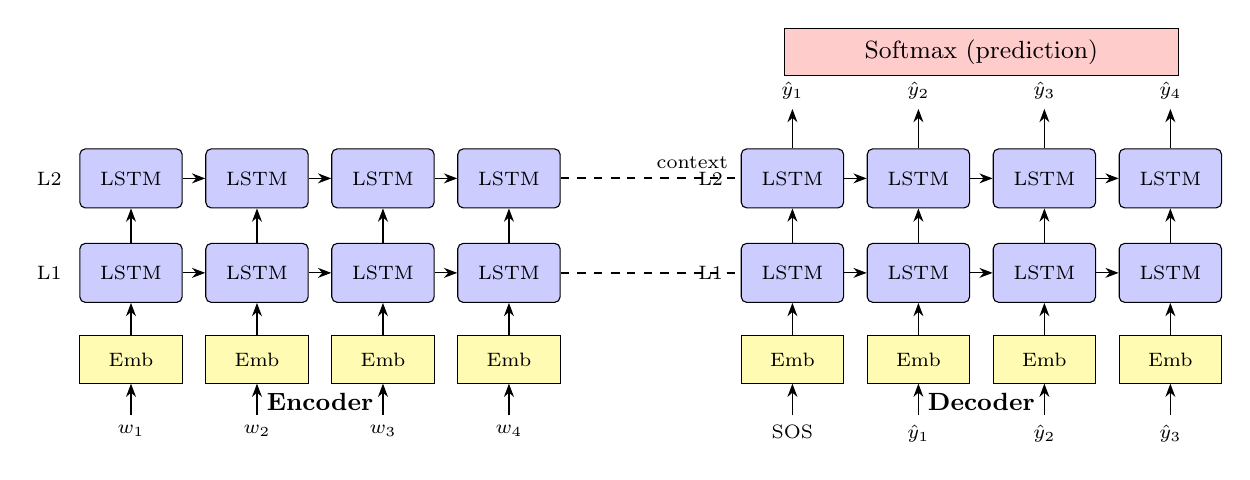
\begin{tikzpicture}[
  lstm/.style={rectangle, draw, fill=blue!20, minimum width=1.3cm,
               minimum height=0.75cm, font=\scriptsize, rounded corners=2pt},
  emb/.style={rectangle, draw, fill=yellow!30, minimum width=1.3cm,
              minimum height=0.6cm, font=\scriptsize},
  sm/.style={rectangle, draw, fill=red!20, minimum width=5cm,
             minimum height=0.6cm, font=\small},
  >=Stealth
]

  %--- ENCODER ---
  \begin{scope}
    % Layer 1
    \foreach \i/\x in {1/0, 2/1.6, 3/3.2, 4/4.8}{
      \node[lstm] (el1\i) at (\x, 0) {LSTM};
    }
    % Layer 2
    \foreach \i/\x in {1/0, 2/1.6, 3/3.2, 4/4.8}{
      \node[lstm] (el2\i) at (\x, 1.2) {LSTM};
    }
    % Embeddings
    \foreach \i/\x in {1/0, 2/1.6, 3/3.2, 4/4.8}{
      \node[emb]  (ee\i)  at (\x, -1.1) {Emb};
    }
    % Inputs
    \foreach \i/\x/\lbl in {1/0/$w_1$, 2/1.6/$w_2$, 3/3.2/$w_3$, 4/4.8/$w_4$}{
      \node[below=0.4cm of ee\i, font=\scriptsize] (ew\i) {\lbl};
      \draw[->] (ew\i) -- (ee\i);
      \draw[->] (ee\i) -- (el1\i);
      \draw[->] (el1\i) -- (el2\i);
    }
    % Recurrent L1
    \draw[->] (el11) -- (el12);
    \draw[->] (el12) -- (el13);
    \draw[->] (el13) -- (el14);
    % Recurrent L2
    \draw[->] (el21) -- (el22);
    \draw[->] (el22) -- (el23);
    \draw[->] (el23) -- (el24);
    % Label
    \node[left=0.1cm of el11, font=\scriptsize, rotate=0] {L1};
    \node[left=0.1cm of el21, font=\scriptsize] {L2};
    \node[below=1.4cm, font=\small\bfseries, xshift=2.4cm] {Encoder};
  \end{scope}

  %--- Context vector ---
  \draw[->, thick, dashed] (el24.east) to[out=0,in=180]
        node[above,font=\scriptsize, xshift=0.2cm]{context} (8.4, 1.2);
  \draw[->, thick, dashed] (el14.east) to[out=0,in=180] (8.4, 0);

  %--- DECODER ---
  \begin{scope}[xshift=8.4cm]
    % Layer 1
    \foreach \i/\x in {1/0, 2/1.6, 3/3.2, 4/4.8}{
      \node[lstm] (dl1\i) at (\x, 0) {LSTM};
    }
    % Layer 2
    \foreach \i/\x in {1/0, 2/1.6, 3/3.2, 4/4.8}{
      \node[lstm] (dl2\i) at (\x, 1.2) {LSTM};
    }
    % Embeddings
    \foreach \i/\x in {1/0, 2/1.6, 3/3.2, 4/4.8}{
      \node[emb]  (de\i)  at (\x, -1.1) {Emb};
    }
    % Inputs
    \foreach \i/\x/\lbl in {1/0/SOS, 2/1.6/$\hat{y}_1$, 3/3.2/$\hat{y}_2$, 4/4.8/$\hat{y}_3$}{
      \node[below=0.4cm of de\i, font=\scriptsize] (dw\i) {\lbl};
      \draw[->] (dw\i) -- (de\i);
      \draw[->] (de\i) -- (dl1\i);
      \draw[->] (dl1\i) -- (dl2\i);
    }
    % Recurrent L1
    \draw[->] (dl11) -- (dl12);
    \draw[->] (dl12) -- (dl13);
    \draw[->] (dl13) -- (dl14);
    % Recurrent L2
    \draw[->] (dl21) -- (dl22);
    \draw[->] (dl22) -- (dl23);
    \draw[->] (dl23) -- (dl24);
    % Output arrows
    \foreach \i in {1,2,3,4}{
      \node[above=0.5cm of dl2\i, font=\scriptsize] (do\i) {$\hat{y}_\i$};
      \draw[->] (dl2\i) -- (do\i);
    }
    % Softmax box
    \node[sm, above=1.3cm] at (2.4, 1.2) (sfm) {Softmax (prediction)};
    % Label
    \node[left=0.1cm of dl11, font=\scriptsize] {L1};
    \node[left=0.1cm of dl21, font=\scriptsize] {L2};
    \node[below=1.4cm, font=\small\bfseries, xshift=2.4cm] {Decoder};
  \end{scope}

\end{tikzpicture}
\caption{Stacked (deep) Seq2Seq architecture with embedding layers
         (Deck \texttt{10-Seq2Seq}, slide 19/25).  Both encoder and decoder
         use two LSTM layers.  The final context vectors from \emph{all} encoder
         layers initialise the corresponding decoder layers.}
\label{fig:stacked_seq2seq}
\end{figure}

\subsubsection*{Context Vector Propagation in Stacked Models}

A common question is whether context vectors from different encoder layers are
equivalent.  They are not.  In a 2-layer encoder:

\begin{align}
  h^{(1)}_t &= \text{LSTM}^{(1)}\!\left(e(x_t),\, h^{(1)}_{t-1}\right),
              \label{eq:enc_l1} \\
  h^{(2)}_t &= \text{LSTM}^{(2)}\!\left(h^{(1)}_t,\, h^{(2)}_{t-1}\right).
              \label{eq:enc_l2}
\end{align}

Layer 2 processes the \emph{transformed} representations from Layer 1 through
a different weight matrix $W^{(2)} \neq W^{(1)}$.  As a result, the context
vector from Layer 2 encodes a higher-level, more abstracted representation than
Layer 1's context vector, even though both are derived from the same source
sentence.

\begin{table}[ht]
\centering
\caption{Effect of architectural choices on Seq2Seq model performance
         (qualitative summary from lecture discussion).}
\label{tab:seq2seq_ablation}
\begin{tabularx}{\textwidth}{lXX}
\toprule
\textbf{Architecture Change} & \textbf{Benefit} & \textbf{Trade-off} \\
\midrule
Raw one-hot input (baseline) &
  Simple to implement &
  High-dimensional, sparse; no semantic similarity captured \\
\addlinespace
+ Embedding layer &
  Dense, learnable representations; semantic proximity captured &
  Additional parameters $d_e \times |\mathcal{V}|$; needs more data \\
\addlinespace
+ Stacked encoder (2 layers) &
  Hierarchical feature extraction; better long-range compression &
  More parameters; slower training \\
\addlinespace
+ Stacked decoder (2 layers) &
  Richer generation capacity &
  Context from \emph{all} encoder layers must initialise decoder layers \\
\addlinespace
+ Teacher forcing &
  Faster convergence during training; more stable gradients &
  Train/test discrepancy (exposure bias); only applicable at train time \\
\bottomrule
\end{tabularx}
\end{table}

\subsection{Limitations of the Basic Seq2Seq Model}
\label{subsec:seq2seq_limitations}

Despite its success, the encoder--decoder Seq2Seq model has two well-known
bottlenecks:

\begin{warningbox}
  \textbf{Context Vector Bottleneck.}  The entire source sequence must be
  compressed into a single fixed-size vector $\mathbf{c}$.  For long
  sentences (beyond $\approx$20--30 tokens), this representation becomes
  information-lossy: early and late words compete for representation in
  the limited vector dimensionality.
\end{warningbox}

\begin{enumerate}
  \item \textbf{Encoder-side bottleneck.}  All $T_x$ source tokens must be
        summarised into $\mathbf{c}$.  Important details from the beginning of
        a long paragraph may be overshadowed by more recent tokens due to the
        recency bias inherent in LSTM.
  \item \textbf{Decoder-side bottleneck.}  The same context vector (with minor
        variations from LSTM processing) is fed at every decoding step.  The
        decoder cannot selectively attend to the most relevant encoder states.
        For example, when generating the Hindi translation of ``I'', only the
        corresponding English token is relevant, not the entire source sentence.
\end{enumerate}

Both limitations are addressed by the \emph{attention mechanism}, which
allows the decoder to dynamically re-weight encoder hidden states at each
decoding step.  This mechanism is discussed in a subsequent session.

%=============================================================
\section{Training Seq2Seq Models: Teacher Forcing}
\label{sec:teacher_forcing}
%=============================================================

\subsection{Training Objective}
\label{subsec:training_obj}

During training, the model minimises the total cross-entropy loss summed over
all target tokens:

\begin{equation}
  \mathcal{L} = -\sum_{t=1}^{T_y} \log P(y_t \mid y_1, \ldots, y_{t-1},\,
                \mathbf{c};\,\theta).
  \label{eq:seq2seq_loss}
\end{equation}

\subsection{Teacher Forcing}
\label{subsec:teacher_forcing}

Without teacher forcing, the decoder receives its own predicted token
$\hat{y}_{t-1}$ as the input at step $t$.  Early in training, $\hat{y}_{t-1}$
is often wrong, causing the error to compound across decoding steps
(\emph{exposure bias}).

\textbf{Teacher forcing} substitutes the model's prediction with the
\emph{ground-truth} target token at each step:

\begin{equation}
  y_t = \text{Decoder}(y^*_{t-1},\, \mathbf{c},\, h^d_{t-1}),
  \label{eq:teacher_forcing}
\end{equation}

where $y^*_{t-1}$ is the ground-truth token at position $t-1$.

\begin{example}[title=Teacher Forcing for English-to-Hindi Translation]
  Suppose the source sentence is ``I am going'' and the target is
  ``Main ja raha hun.'' Without teacher forcing, if the decoder incorrectly
  predicts ``who'' as the first token, this wrong token propagates as input
  to the next step, compounding the error.  With teacher forcing, the correct
  token ``Main'' is fed at each step regardless of the model's prediction,
  enabling faster and more stable training convergence.
\end{example}

\begin{remark}
  \label{rem:teacher_forcing_inference}
  Teacher forcing is applied \emph{exclusively at training time}.  During
  inference (test time), the ground-truth sequence is unavailable, so the model
  operates auto-regressively: $\hat{y}_{t-1}$ is fed as input at step $t$.
\end{remark}

\begin{algorithm}[H]
\caption{Seq2Seq Training with Teacher Forcing}
\label{alg:seq2seq_train}
\SetAlgoLined
\KwIn{Source sequence $\mathbf{x}$, target sequence $\mathbf{y}^*$,
      model parameters $\theta$, learning rate $\eta$}
\KwOut{Updated parameters $\theta$}
\BlankLine
$\mathbf{c} = (h^e_{T_x}, c^e_{T_x}) \leftarrow \text{Encoder}(\mathbf{x};\,\theta_{\text{enc}})$\;
$h^d_0 \leftarrow h^e_{T_x}$,\quad $c^d_0 \leftarrow c^e_{T_x}$\;
$\mathcal{L} \leftarrow 0$\;
\For{$t = 1$ \KwTo $T_y$}{
  $\hat{y}_t,\, h^d_t,\, c^d_t \leftarrow
    \text{Decoder}\!\left(y^*_{t-1},\, h^d_{t-1},\, c^d_{t-1};\,
    \theta_{\text{dec}}\right)$\;
  $\mathcal{L} \leftarrow \mathcal{L} - \log P(y^*_t \mid \hat{y}_t)$\;
}
Back-propagate $\nabla_\theta \mathcal{L}$ through time\;
$\theta \leftarrow \theta - \eta \nabla_\theta \mathcal{L}$\;
\Return $\theta$\;
\end{algorithm}

%=============================================================
\section{Hands-On: Seq2Seq Implementation in PyTorch}
\label{sec:handson}
%=============================================================

The hands-on portion of Session 23 used
\texttt{dl-NTSeqToSeqModels.ipynb} (Google Colab) to build an
English-to-Hindi Seq2Seq pipeline from scratch.

\subsection{Dataset}
\label{subsec:dataset}

The dataset contains parallel English--Hindi sentence pairs sourced from
Kaggle (English-to-Hindi Machine Translation dataset).  Key statistics:

\begin{itemize}
  \item Total rows (after NaN removal): $\approx 1{,}77{,}006$.
  \item Training sample used in session: 10{,}000 rows (for computational
        tractability on a Colab CPU instance).
  \item Columns: \texttt{English sentence}, \texttt{Hindi sentence}.
\end{itemize}

\subsection{Data Preprocessing Pipeline}
\label{subsec:preprocessing}

The preprocessing pipeline follows five stages:

\begin{enumerate}
  \item \textbf{Data cleaning.}  Drop rows with missing values
        (\texttt{dropna}) and reset the index.
  \item \textbf{Type conversion.}  Convert each column to \texttt{str} and
        then to a list of token strings to handle mixed-type entries.
  \item \textbf{Tokenisation.}  Lowercase, strip whitespace, and split on
        spaces.
  \item \textbf{Vocabulary construction.}  Assign a unique integer index to
        each unique token.  Four special tokens are reserved:
        \texttt{PAD} (0), \texttt{UNK} (1), \texttt{SOS} (2), \texttt{EOS} (3).
  \item \textbf{Encoding.}  Map each sentence to a sequence of token indices.
        Hindi decoder sequences are prefixed with \texttt{SOS} and suffixed
        with \texttt{EOS}.
\end{enumerate}

\begin{codebox}[title=Tokenisation Function (Python)]
\begin{verbatim}
def tokenize(sentence):
    if not isinstance(sentence, str):
        return []
    return sentence.lower().strip().split()
\end{verbatim}
\end{codebox}

\subsubsection*{Vocabulary Sizes}

After processing 10{,}000 sentence pairs:
\begin{itemize}
  \item English vocabulary: $\approx 22{,}000$ unique tokens.
  \item Hindi vocabulary:   $\approx 24{,}000$ unique tokens.
\end{itemize}

The two vocabularies are entirely separate; the model uses the English
vocabulary at encode time and the Hindi vocabulary at decode time, so there is
no index collision.

\subsection{Padding for Batching}
\label{subsec:padding}

Because sentences in a batch differ in length, all sequences must be padded to
a common maximum length \texttt{MAX\_LEN} before being stacked into tensors.

\begin{codebox}[title=Padding Function (Python -- from slide V04)]
\begin{verbatim}
def pad_sequence(seq, max_len, pad_value=0):
    if len(seq) < max_len:
        seq = seq + [pad_value] * (max_len - len(seq))
    return seq

# Compute MAX_LEN across encoder and decoder sequences
MAX_LEN = max([len(s) for s in encoded_inputs])
MAX_LEN = max(MAX_LEN, max([len(s) for s in encoded_outputs]))
print("Max Sequence Length:", MAX_LEN)
\end{verbatim}
\end{codebox}

\begin{keyinsight}
  \texttt{MAX\_LEN} is computed as the maximum length \emph{across both encoder
  and decoder sequences}.  This ensures that the padding dimension is
  consistent for both the source and target batch tensors, which simplifies
  batching in the \texttt{DataLoader}.
\end{keyinsight}

The padding token index is 0 (\texttt{PAD}).  The model ignores padded
positions either through a padding mask or via PyTorch's
\texttt{pack\_padded\_sequence} utility, which avoids feeding padding tokens
to the LSTM.

\subsection{Encoder Implementation}
\label{subsec:encoder_impl}

The \texttt{Encoder} class wraps a single \texttt{nn.Embedding} layer followed
by an \texttt{nn.LSTM}:

\begin{codebox}[title=Encoder Hyperparameters and Instantiation (V05)]
\begin{verbatim}
EMBEDDING_DIM = 128
HIDDEN_DIM    = 256
ENCODER_DIM   = HIDDEN_DIM
DECODER_DIM   = HIDDEN_DIM

encoder = Encoder(
    input_dim    = len(encoder_vocab),
    embedding_dim = EMBEDDING_DIM,
    hidden_dim   = HIDDEN_DIM,
    n_layers     = 1,
    dropout      = 0
)
\end{verbatim}
\end{codebox}

\subsubsection*{Sanity Check}

After a forward pass on one batch from \texttt{train\_loader}:

\begin{codebox}[title=Encoder Sanity Check]
\begin{verbatim}
for src_batch, tgt_batch in train_loader:
    e_h, e_c = encoder(src_batch)
    print("e_h shape:", e_h.shape)  # torch.Size([1, 128, 256])
    print("e_c shape:", e_c.shape)  # torch.Size([1, 128, 256])
    break

# Remove layer dimension for decoder initialisation
context_h = e_h.squeeze(0)  # shape: [128, 256]
context_c = e_c.squeeze(0)  # shape: [128, 256]
\end{verbatim}
\end{codebox}

The output tensors have shape $[\texttt{n\_layers},\,\texttt{batch\_size},\,
\texttt{hidden\_dim}]$, i.e., $[1, 128, 256]$.  The \texttt{.squeeze(0)} call
removes the \texttt{n\_layers} dimension, yielding context vectors of shape
$[128, 256]$ that are ready to initialise the decoder's initial hidden and cell
states.

\begin{remark}
  \label{rem:nlayers}
  For a stacked encoder with \texttt{n\_layers = 2}, the output tensors have
  shape $[2, 128, 256]$.  The decoder must also have 2 layers, and
  \texttt{e\_h[0]} and \texttt{e\_h[1]} initialise the first and second
  decoder LSTM layers respectively.
\end{remark}

\subsection{Tensor Shape Summary}
\label{subsec:shapes}

\begin{table}[ht]
\centering
\caption{Tensor shapes at key stages of the Seq2Seq pipeline
         (batch size $B=128$, embedding dim $d_e=128$, hidden dim
         $d_h=256$, vocabulary size $|\mathcal{V}|$).}
\label{tab:tensor_shapes}
\begin{tabularx}{\textwidth}{lXl}
\toprule
\textbf{Tensor} & \textbf{Description} & \textbf{Shape} \\
\midrule
\texttt{src\_batch}    & Padded encoder input token IDs & $[B, T_x]$ \\
\texttt{tgt\_batch}    & Padded decoder input token IDs & $[B, T_y]$ \\
\texttt{embedding}     & Embedded encoder input         & $[B, T_x, d_e]$ \\
\texttt{lstm\_out}     & LSTM hidden states (all steps) & $[B, T_x, d_h]$ \\
\texttt{e\_h}          & Encoder final hidden state     & $[\texttt{n\_layers}, B, d_h]$ \\
\texttt{e\_c}          & Encoder final cell state       & $[\texttt{n\_layers}, B, d_h]$ \\
\texttt{context\_h}    & After \texttt{.squeeze(0)}     & $[B, d_h]$ \\
\texttt{decoder\_out}  & Decoder output logits          & $[B, T_y, |\mathcal{V}|]$ \\
\bottomrule
\end{tabularx}
\end{table}

\subsection{Special Tokens}
\label{subsec:special_tokens}

Four special tokens are defined and reserved before building the vocabulary:

\begin{itemize}
  \item \textbf{PAD} (index 0): padding token, used to fill shorter sequences.
  \item \textbf{UNK} (index 1): unknown token, used for out-of-vocabulary words.
  \item \textbf{SOS} (index 2): start-of-sequence token, prepended to every
        decoder input sequence.
  \item \textbf{EOS} (index 3): end-of-sequence token, appended to every
        decoder target sequence.  At inference time, the decoder stops
        generating when it predicts \texttt{EOS}.
\end{itemize}

\begin{example}[title=Decoder Sequence Construction]
  For the Hindi sentence ``Main ja raha hun'', the decoder input and target
  sequences are constructed as:
  \begin{align*}
    \text{Decoder input:}  &\quad [\texttt{SOS},\, \text{Main},\, \text{ja},\,
                                   \text{raha},\, \text{hun}] \\
    \text{Decoder target:} &\quad [\text{Main},\, \text{ja},\, \text{raha},\,
                                   \text{hun},\, \texttt{EOS}]
  \end{align*}
  The model is trained to predict the target sequence given the decoder input,
  implementing a next-token prediction (auto-regressive) objective.
\end{example}

%=============================================================
\section{Connecting Bidirectionality and Seq2Seq}
\label{sec:connection}
%=============================================================

The Bidirectional RNN and Seq2Seq architectures serve complementary roles.
The table below summarises key differences and the relationship between the two.

\begin{table}[ht]
\centering
\caption{Bidirectional RNN vs.\ Seq2Seq: architectural comparison.}
\label{tab:birnn_vs_seq2seq}
\begin{tabularx}{\textwidth}{lXX}
\toprule
\textbf{Aspect} & \textbf{Bidirectional RNN} & \textbf{Seq2Seq} \\
\midrule
Input / Output &
  Sequence $\to$ Sequence (same length) &
  Sequence $\to$ Sequence (different lengths) \\
Context &
  Full past + future at each position &
  Encoder compresses full source; decoder uses context vector \\
Typical role &
  Encoder for classification / labelling &
  Encoder--Decoder for generation tasks \\
Bidirectionality &
  Core architectural feature &
  Can use Bi-RNN as the encoder; decoder must be unidirectional \\
Applications &
  NER, POS, QA, BERT pre-training &
  MT, summarisation, ASR, image captioning \\
\bottomrule
\end{tabularx}
\end{table}

A natural combination is to use a \textbf{Bidirectional LSTM as the encoder}
within a Seq2Seq model.  The encoder then produces context vectors

\begin{equation}
  \mathbf{c} = \left[\overrightarrow{h}_{T_x};\;\overleftarrow{h}_{T_x}\right]
              \in \mathbb{R}^{2d_h},
  \label{eq:bienc_context}
\end{equation}

which are then projected down to $d_h$ before initialising the (unidirectional)
decoder.

\begin{keyinsight}
  The BERT model (Devlin et al., 2018) is essentially a \emph{deeply stacked
  bidirectional encoder} trained with a masked language modelling objective.
  The GPT family of models uses a deeply stacked unidirectional decoder trained
  with a causal language modelling objective.  These two design choices reflect
  the encoder/decoder split described in this session.
\end{keyinsight}

%=============================================================
\section{Summary and Conclusion}
\label{sec:conclusion}
%=============================================================

Session 23 presented a coherent progression through three related topics:

\begin{enumerate}
  \item \textbf{Bidirectional RNN.}  Two independent recurrent chains (forward
        and backward) process the same input sequence simultaneously.  At each
        position, both hidden states are concatenated to form the output
        $y_t = [\overrightarrow{h}_t;\,\overleftarrow{h}_t]$.  This gives the
        model access to both past and future context, making it well-suited for
        tasks such as Named Entity Recognition, POS tagging, and fill-in-the-blank
        prediction.  Bidirectionality is unsuitable for causal tasks (language
        modelling, streaming speech) where future tokens are not available.

  \item \textbf{Seq2Seq with Stacked Layers and Embeddings.}  The basic
        encoder--decoder LSTM architecture is enhanced by: (a) replacing
        one-hot inputs with dense embedding vectors, and (b) stacking multiple
        LSTM layers in both encoder and decoder.  Each additional layer learns
        progressively more abstract representations.  The context vectors from
        the encoder's final hidden and cell states initialise the decoder.
        Training uses teacher forcing, which substitutes the ground-truth target
        token as decoder input at each step, accelerating convergence.

  \item \textbf{Hands-On Implementation.}  The Colab notebook demonstrated the
        full English-to-Hindi translation pipeline: dataset loading and cleaning,
        tokenisation, dual-vocabulary construction, index encoding with SOS/EOS
        tokens, padding to \texttt{MAX\_LEN}, and the \texttt{Encoder} class
        with \texttt{nn.Embedding} and \texttt{nn.LSTM}.  The sanity check
        confirmed output shapes $[1, 128, 256]$ for both hidden and cell states;
        \texttt{.squeeze(0)} reduces these to $[128, 256]$ context vectors for
        decoder initialisation.
\end{enumerate}

\subsubsection*{Limitations and Next Steps}

The session also highlighted the \emph{context-vector bottleneck}: compressing
an arbitrarily long source sentence into a single fixed-size vector degrades
performance as sentence length increases.  The solution --- the \emph{attention
mechanism}~\cite{bahdanau2015neural} --- allows the decoder to attend to all
encoder hidden states dynamically at each decoding step, and will be the focus
of the next session.

\subsubsection*{Key Equations Summary}

\begin{align}
  \text{Bi-RNN output:} \quad
  y_t &= \left[\overrightarrow{h}_t;\;\overleftarrow{h}_t\right] \tag{\ref{eq:birnn_output}} \\
  \text{Embedding:} \quad
  e_i &= E\cdot\mathbf{1}_i \in \mathbb{R}^{d_e} \tag{\ref{eq:embedding}} \\
  \text{Encoder context:} \quad
  \mathbf{c} &= (h^e_{T_x},\, c^e_{T_x}) \tag{\ref{eq:encoder}} \\
  \text{Training loss:} \quad
  \mathcal{L} &= -\sum_{t=1}^{T_y}
    \log P(y_t \mid y^*_1, \ldots, y^*_{t-1}, \mathbf{c};\,\theta)
    \tag{\ref{eq:seq2seq_loss}}
\end{align}

%=============================================================
% References (manually listed; use bibtex in production)
%=============================================================
\begin{thebibliography}{9}

\bibitem{schuster1997bidirectional}
M.\ Schuster and K.\ K.\ Paliwal,
``Bidirectional recurrent neural networks,''
\textit{IEEE Transactions on Signal Processing},
vol.~45, no.~11, pp.~2673--2681, 1997.

\bibitem{hochreiter1997long}
S.\ Hochreiter and J.\ Schmidhuber,
``Long short-term memory,''
\textit{Neural Computation},
vol.~9, no.~8, pp.~1735--1780, 1997.

\bibitem{cho2014learning}
K.\ Cho, B.\ van Merrienboer, C.\ Gulcehre, D.\ Bahdanau, F.\ Bougares,
H.\ Schwenk, and Y.\ Bengio,
``Learning phrase representations using RNN encoder--decoder for statistical
machine translation,''
in \textit{Proc.\ EMNLP}, 2014, pp.~1724--1734.

\bibitem{sutskever2014sequence}
I.\ Sutskever, O.\ Vinyals, and Q.\ V.\ Le,
``Sequence to sequence learning with neural networks,''
in \textit{Advances in Neural Information Processing Systems (NeurIPS)},
vol.~27, 2014.

\bibitem{bahdanau2015neural}
D.\ Bahdanau, K.\ Cho, and Y.\ Bengio,
``Neural machine translation by jointly learning to align and translate,''
in \textit{Proc.\ ICLR}, 2015.

\bibitem{devlin2019bert}
J.\ Devlin, M.-W.\ Chang, K.\ Lee, and K.\ Toutanova,
``BERT: Pre-training of deep bidirectional transformers for language
understanding,''
in \textit{Proc.\ NAACL-HLT}, 2019, pp.~4171--4186.

\bibitem{saumya2026slides}
S.\ Saumya and S.\ R.\ M.\ Prasanna,
\textit{Deep Learning Lecture Slides -- Session 23: 05-DL-RNN \&
10-Seq2Seq},
Indian Institute of Information Technology Dharwad, February 2026.

\end{thebibliography}

\clearpage

\end{document}
